

%!TEX root = /Users/sbogutzky/Entwicklung/projects/bogutzky/repositories/2939413/final-draft.tex
\section{Flow und Laufen (intraindividuell)} 

% (fold)
\label{sec:flow_und_laufen_intraindividuell}

\section{Einleitung} % (fold)
\label{sec:einleitung_5_1}

Ziel der in diesem Abschnitt beschriebenen Studie war es, zu untersuchen, ob subjektive, durch Experience Sampling erhobene, Flow-Merkmale mit den nachfolgenden Kandidaten für ein implizites Messverfahren des Flow-Erlebens beim Laufen in einem Zusammenhang stehen (Abschnitt~\ref{sec:herangehensweise}, Schritt 2):

\begin{itemize}
	\item mittlere \ac{HR}
	\item \acs{RMSSD} der zeitbezogenen statitischen \ac{HRV}-Analyse
	\item Bewegungsaufwand (Abschnitt~\ref{ssub:der_bewegungsfluss}) oder
	\item normalisierter Shannon Entropie Index der kardio-lokomotorischen Phasensynchronisation (Abschnitt~\ref{ssub:die_kardio_lokomotorische_phasensynchronisation})
\end{itemize}

Die Auswahl der Merkmale begründe ich durch:

\begin{enumerate}
	\item ihre nachgewiesenen Zusammenhänge zum Flow-Erleben bei Tätigkeiten mit geringer physischer Beansprung (Abschnitt~\ref{ssub:kardiovaskulare_messungen}) 
	\item die Praktikabilität bei der Ausführung einer physisch belastenden Tätigkeit
\end{enumerate}

Aufgrund der durch das \acs{BMBF}-Projekt bereitgestellten Shimmer \acp{IMU}, nutzte ich ein Shimmer EKG-Modul, das auf die Hauptplatine einer Shimmer \ac{IMU} aufgesetzt wird. Das Shimmer EKG-Modul arbeitet mit der Ableitung nach Einthoven \citep[][S.~85ff.]{Behrends2002}. Es handelt sich um eine bipolare Extremitätenableitung, die man routinemäßig mit drei Elektroden plus einer Erdungselektrode erfasst. Ich platzierte vier konventionelle Einwegelektroden auf der Körperoberfläche und verband sie mit vier Kabelverbindungen mit dem Shimmer EKG-Modul wie in Abbildung~\ref{fig:5_1_equipment_setup} dargestellt. Damit erfasst das Shimmer EKG-Modul mit zwei Kanälen die zwei Ableitungen (II-III). Ableitung I berechnete ich, indem ich das Signal von LA-LL von dem Signal von RA-LL subtrahiere.

\begin{itemize}
	\item Ableitung I: zwischen rechtem und linkem Arm (RA-LA)
	\item Ableitung II: zwischen rechtem Arm und linkem Bein (RA-LL)
	\item Ableitung III: zwischen linkem Arm und linkem Bein (LA-LL)
\end{itemize}

Die Ableitung nach Einthoven dient zur Darstellung von Potenzialänderungen in der Frontalebene und ermöglicht u. a. die Identifikation von Herzschlägen, die wir zur Analyse der \ac{HRV} benötigen.

Wie in Abschnitt~\ref{ssub:kardiovaskulare_messungen} zusammengefasst, handelt es sich bei der \acs{RMSSD} um ein physiologisches Merkmal der zeitbezogenen statitischen \ac{HRV}-Analyse, mit dem \citet{Keller2011} bei einer sitzenden Tätigkeit Zusammenhänge mit Flow-Erleben feststellten. Auf Zusammenhanganalysen mit frequenzbezogenen \ac{HRV}-Merkmalen verzichtete ich aufgrund der in Abschnitt~\ref{sub:zuordnung} beschriebenen Probleme.

Kinematische Daten maß ich mit den bereitgestellten Shimmer \acp{IMU} und einem zusätzlichen Shimmer Gyro-Modul. Die kinematischen Daten benötigte ich, um einzelne sich wiederholende Bewegungsabläufe der Bewegung zu erkennen und den Bewegungsaufwand zu berechnen. Zusätzliche kinematische Merkmale, die z.~B. Abschnitt~\ref{sub:lauftechnik_detektionstechnologie} beschreibt, berücksichtigte ich nicht.

Die Anordnung des Equipments und die Zuverlässigkeit der Datenaufzeichnung testete ich in Vorab-Tests mit drei Freiwilligen aus der Fakultät 4 der Hochschule Bremen. Für die Vorab-Tests verwendete ich denselben Aufbau des Systems, der bei dieser Studie zum Einsatz kam (siehe Abschnitt~\ref{sub:apparat}).

\begin{figure}[t]
	\centering
		\includegraphics[width=1.00\textwidth]{5_1_equipment_setup}
	\caption[Equipment der ersten Studie zum Flow-Erleben beim Laufen]{Equipment der ersten Studie zum Flow-Erleben beim Laufen}
	\label{fig:5_1_equipment_setup}
\end{figure}

% section einleitung (end)

\section{Methode} % (fold)
\label{sec:methode}

\citet[][S.~989]{Strohrmann2012} argumentieren, Untersuchungen in Außen-Umgebungen durchzuführen, da sich das Laufen auf einem Laufband von dem Laufen in Außen-Umgebungen in Bezug auf kinematische Merkmale unterscheidet. Aus dem genannten Grund entschied ich mich, die Läufe unter realen Bedingungen durchzuführen. Untersuchungen außerhalb von Laboratorien stellen bei ihrer Durchführung eine Herausforderung dar. Außen-Umgebungen sind in einem hohen Maße veränderlich und kontextsensitive Faktoren als Einflüsse auf Merkmale sind grundsätzlich als gegeben anzunehmen. Gleichwohl sind solche Untersuchungen unerlässlich, um eine realistischere Einschätzung der Nutzung in Außen-Umgebungen zu ermöglichen.

Für die in diesem Abschnitt dokumentierte Studie setzte ich ein Echtzeit-Datenerfassungsverfahren (real-time data capture) ein. Die Datenerfassung umfasst \ac{EKG}-Daten und kinematische Daten sowie Selbstauskünfte durch die \ac{FKS}. Die aufgezeichneten Datenströme eines einzelnen Bewegungsablaufs beim Laufen sind in Abbildung~\ref{fig:5_2_daten} dargestellt. Der Bewegungsablauf beginnt und endet mit dem mittleren Schwung des rechten Beines (negative Signalspitze der Winkelgeschwindigkeit um die X-Achse (grün)).

\begin{sidewaysfigure}
	\resizebox{1.00\textwidth}{!}{%
	    % Created by tikzDevice version 0.10.1 on 2016-08-31 09:50:34
% !TEX encoding = UTF-8 Unicode
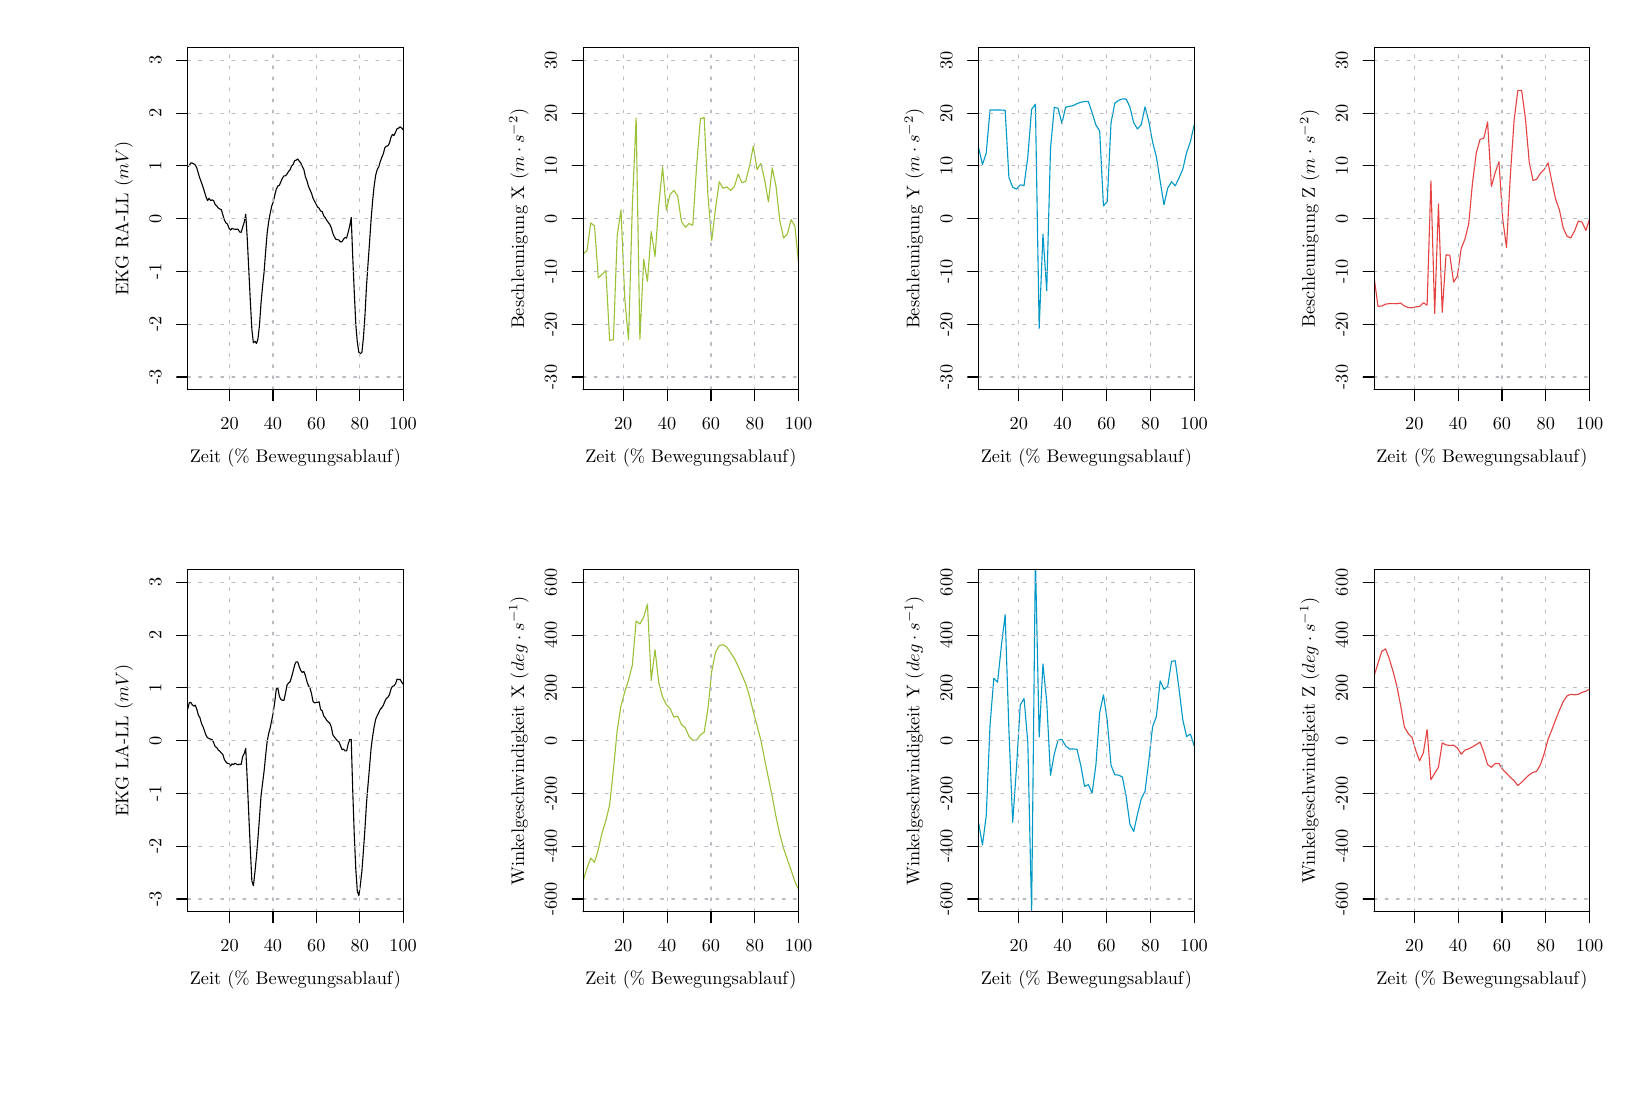
\begin{tikzpicture}[x=1pt,y=1pt]
\definecolor{fillColor}{RGB}{255,255,255}
\path[use as bounding box,fill=fillColor,fill opacity=0.00] (0,0) rectangle (571.66,377.25);
\begin{scope}
\path[clip] ( 57.82,246.44) rectangle (135.69,370.02);
\definecolor{drawColor}{RGB}{0,0,0}

\path[draw=drawColor,line width= 0.4pt,line join=round,line cap=round] ( 57.82,327.07) --
	( 58.37,327.42) --
	( 58.92,328.37) --
	( 59.47,328.34) --
	( 60.03,328.02) --
	( 60.58,327.61) --
	( 61.13,326.47) --
	( 61.68,324.55) --
	( 62.23,322.80) --
	( 62.79,321.29) --
	( 63.34,319.69) --
	( 63.89,317.94) --
	( 64.44,316.10) --
	( 65.00,314.78) --
	( 65.55,315.58) --
	( 66.10,314.77) --
	( 66.65,315.02) --
	( 67.20,314.76) --
	( 67.76,313.33) --
	( 68.31,312.86) --
	( 68.86,312.06) --
	( 69.41,311.74) --
	( 69.97,311.49) --
	( 70.52,309.65) --
	( 71.07,307.74) --
	( 71.62,306.71) --
	( 72.18,306.31) --
	( 72.73,304.87) --
	( 73.28,304.08) --
	( 73.83,304.72) --
	( 74.38,304.48) --
	( 74.94,304.40) --
	( 75.49,304.40) --
	( 76.04,304.40) --
	( 76.59,303.44) --
	( 77.15,303.28) --
	( 77.70,305.19) --
	( 78.25,306.94) --
	( 78.80,309.84) --
	( 79.35,300.97) --
	( 79.91,289.48) --
	( 80.46,278.47) --
	( 81.01,268.23) --
	( 81.56,263.38) --
	( 82.12,263.92) --
	( 82.67,263.13) --
	( 83.22,264.83) --
	( 83.77,269.81) --
	( 84.33,277.78) --
	( 84.88,283.80) --
	( 85.43,288.96) --
	( 85.98,296.28) --
	( 86.53,302.94) --
	( 87.09,307.21) --
	( 87.64,310.17) --
	( 88.19,312.82) --
	( 88.74,314.26) --
	( 89.30,316.79) --
	( 89.85,318.89) --
	( 90.40,320.04) --
	( 90.95,320.27) --
	( 91.50,321.60) --
	( 92.06,322.89) --
	( 92.61,323.71) --
	( 93.16,323.72) --
	( 93.71,324.33) --
	( 94.27,325.29) --
	( 94.82,325.92) --
	( 95.37,327.28) --
	( 95.92,327.84) --
	( 96.48,329.20) --
	( 97.03,329.38) --
	( 97.58,329.79) --
	( 98.13,329.02) --
	( 98.68,328.39) --
	( 99.24,327.04) --
	( 99.79,326.04) --
	(100.34,323.42) --
	(100.89,322.03) --
	(101.45,319.98) --
	(102.00,318.66) --
	(102.55,317.49) --
	(103.10,315.65) --
	(103.65,314.58) --
	(104.21,313.48) --
	(104.76,312.41) --
	(105.31,312.02) --
	(105.86,310.98) --
	(106.42,310.83) --
	(106.97,309.27) --
	(107.52,308.58) --
	(108.07,307.65) --
	(108.63,306.83) --
	(109.18,306.13) --
	(109.73,304.91) --
	(110.28,302.91) --
	(110.83,301.67) --
	(111.39,300.76) --
	(111.94,300.64) --
	(112.49,300.52) --
	(113.04,299.80) --
	(113.60,299.96) --
	(114.15,300.82) --
	(114.70,301.45) --
	(115.25,301.22) --
	(115.80,303.29) --
	(116.36,305.59) --
	(116.91,308.64) --
	(117.46,294.43) --
	(118.01,281.80) --
	(118.57,269.92) --
	(119.12,263.62) --
	(119.67,259.93) --
	(120.22,259.45) --
	(120.78,259.95) --
	(121.33,265.34) --
	(121.88,273.27) --
	(122.43,283.79) --
	(122.98,291.89) --
	(123.54,299.70) --
	(124.09,307.90) --
	(124.64,314.58) --
	(125.19,320.03) --
	(125.75,323.95) --
	(126.30,325.93) --
	(126.85,326.95) --
	(127.40,328.81) --
	(127.96,330.39) --
	(128.51,331.69) --
	(129.06,333.87) --
	(129.61,334.43) --
	(130.16,334.53) --
	(130.72,335.53) --
	(131.27,337.59) --
	(131.82,338.65) --
	(132.37,338.31) --
	(132.93,339.44) --
	(133.48,340.74) --
	(134.03,340.94) --
	(134.58,341.42) --
	(135.13,341.04) --
	(135.69,340.33);
\end{scope}
\begin{scope}
\path[clip] (  0.00,  0.00) rectangle (571.66,377.25);
\definecolor{drawColor}{RGB}{0,0,0}

\path[draw=drawColor,line width= 0.4pt,line join=round,line cap=round] ( 72.95,246.44) -- (135.69,246.44);

\path[draw=drawColor,line width= 0.4pt,line join=round,line cap=round] ( 72.95,246.44) -- ( 72.95,242.48);

\path[draw=drawColor,line width= 0.4pt,line join=round,line cap=round] ( 88.63,246.44) -- ( 88.63,242.48);

\path[draw=drawColor,line width= 0.4pt,line join=round,line cap=round] (104.32,246.44) -- (104.32,242.48);

\path[draw=drawColor,line width= 0.4pt,line join=round,line cap=round] (120.00,246.44) -- (120.00,242.48);

\path[draw=drawColor,line width= 0.4pt,line join=round,line cap=round] (135.69,246.44) -- (135.69,242.48);

\node[text=drawColor,anchor=base,inner sep=0pt, outer sep=0pt, scale=  0.66] at ( 72.95,232.18) {20};

\node[text=drawColor,anchor=base,inner sep=0pt, outer sep=0pt, scale=  0.66] at ( 88.63,232.18) {40};

\node[text=drawColor,anchor=base,inner sep=0pt, outer sep=0pt, scale=  0.66] at (104.32,232.18) {60};

\node[text=drawColor,anchor=base,inner sep=0pt, outer sep=0pt, scale=  0.66] at (120.00,232.18) {80};

\node[text=drawColor,anchor=base,inner sep=0pt, outer sep=0pt, scale=  0.66] at (135.69,232.18) {100};

\path[draw=drawColor,line width= 0.4pt,line join=round,line cap=round] ( 57.82,251.02) -- ( 57.82,365.45);

\path[draw=drawColor,line width= 0.4pt,line join=round,line cap=round] ( 57.82,251.02) -- ( 53.86,251.02);

\path[draw=drawColor,line width= 0.4pt,line join=round,line cap=round] ( 57.82,270.09) -- ( 53.86,270.09);

\path[draw=drawColor,line width= 0.4pt,line join=round,line cap=round] ( 57.82,289.16) -- ( 53.86,289.16);

\path[draw=drawColor,line width= 0.4pt,line join=round,line cap=round] ( 57.82,308.23) -- ( 53.86,308.23);

\path[draw=drawColor,line width= 0.4pt,line join=round,line cap=round] ( 57.82,327.30) -- ( 53.86,327.30);

\path[draw=drawColor,line width= 0.4pt,line join=round,line cap=round] ( 57.82,346.37) -- ( 53.86,346.37);

\path[draw=drawColor,line width= 0.4pt,line join=round,line cap=round] ( 57.82,365.45) -- ( 53.86,365.45);

\node[text=drawColor,rotate= 90.00,anchor=base,inner sep=0pt, outer sep=0pt, scale=  0.66] at ( 48.31,251.02) {-3};

\node[text=drawColor,rotate= 90.00,anchor=base,inner sep=0pt, outer sep=0pt, scale=  0.66] at ( 48.31,270.09) {-2};

\node[text=drawColor,rotate= 90.00,anchor=base,inner sep=0pt, outer sep=0pt, scale=  0.66] at ( 48.31,289.16) {-1};

\node[text=drawColor,rotate= 90.00,anchor=base,inner sep=0pt, outer sep=0pt, scale=  0.66] at ( 48.31,308.23) {0};

\node[text=drawColor,rotate= 90.00,anchor=base,inner sep=0pt, outer sep=0pt, scale=  0.66] at ( 48.31,327.30) {1};

\node[text=drawColor,rotate= 90.00,anchor=base,inner sep=0pt, outer sep=0pt, scale=  0.66] at ( 48.31,346.37) {2};

\node[text=drawColor,rotate= 90.00,anchor=base,inner sep=0pt, outer sep=0pt, scale=  0.66] at ( 48.31,365.45) {3};

\path[draw=drawColor,line width= 0.4pt,line join=round,line cap=round] ( 57.82,246.44) --
	(135.69,246.44) --
	(135.69,370.02) --
	( 57.82,370.02) --
	( 57.82,246.44);
\end{scope}
\begin{scope}
\path[clip] (  0.00,188.62) rectangle (142.91,377.25);
\definecolor{drawColor}{RGB}{0,0,0}

\node[text=drawColor,anchor=base,inner sep=0pt, outer sep=0pt, scale=  0.66] at ( 96.75,220.30) {Zeit (\% Bewegungsablauf)};

\node[text=drawColor,rotate= 90.00,anchor=base,inner sep=0pt, outer sep=0pt, scale=  0.66] at ( 36.43,308.23) {EKG RA-LL ($mV$)};
\end{scope}
\begin{scope}
\path[clip] ( 57.82,246.44) rectangle (135.69,370.02);
\definecolor{drawColor}{RGB}{186,187,194}

\path[draw=drawColor,line width= 0.4pt,dash pattern=on 1pt off 3pt ,line join=round,line cap=round] ( 72.95,246.44) -- ( 72.95,370.02);

\path[draw=drawColor,line width= 0.4pt,dash pattern=on 1pt off 3pt ,line join=round,line cap=round] ( 88.63,246.44) -- ( 88.63,370.02);

\path[draw=drawColor,line width= 0.4pt,dash pattern=on 1pt off 3pt ,line join=round,line cap=round] (104.32,246.44) -- (104.32,370.02);

\path[draw=drawColor,line width= 0.4pt,dash pattern=on 1pt off 3pt ,line join=round,line cap=round] (120.00,246.44) -- (120.00,370.02);

\path[draw=drawColor,line width= 0.4pt,dash pattern=on 1pt off 3pt ,line join=round,line cap=round] (135.69,246.44) -- (135.69,370.02);

\path[draw=drawColor,line width= 0.4pt,dash pattern=on 1pt off 3pt ,line join=round,line cap=round] ( 57.82,251.02) -- (135.69,251.02);

\path[draw=drawColor,line width= 0.4pt,dash pattern=on 1pt off 3pt ,line join=round,line cap=round] ( 57.82,270.09) -- (135.69,270.09);

\path[draw=drawColor,line width= 0.4pt,dash pattern=on 1pt off 3pt ,line join=round,line cap=round] ( 57.82,289.16) -- (135.69,289.16);

\path[draw=drawColor,line width= 0.4pt,dash pattern=on 1pt off 3pt ,line join=round,line cap=round] ( 57.82,308.23) -- (135.69,308.23);

\path[draw=drawColor,line width= 0.4pt,dash pattern=on 1pt off 3pt ,line join=round,line cap=round] ( 57.82,327.30) -- (135.69,327.30);

\path[draw=drawColor,line width= 0.4pt,dash pattern=on 1pt off 3pt ,line join=round,line cap=round] ( 57.82,346.37) -- (135.69,346.37);

\path[draw=drawColor,line width= 0.4pt,dash pattern=on 1pt off 3pt ,line join=round,line cap=round] ( 57.82,365.45) -- (135.69,365.45);
\end{scope}
\begin{scope}
\path[clip] (  0.00,  0.00) rectangle (571.66,377.25);
\definecolor{drawColor}{RGB}{0,0,0}

\path[draw=drawColor,line width= 0.4pt,line join=round,line cap=round] ( 57.82,246.44) --
	(135.69,246.44) --
	(135.69,370.02) --
	( 57.82,370.02) --
	( 57.82,246.44);
\end{scope}
\begin{scope}
\path[clip] ( 57.82, 57.82) rectangle (135.69,181.40);
\definecolor{drawColor}{RGB}{0,0,0}

\path[draw=drawColor,line width= 0.4pt,line join=round,line cap=round] ( 57.82,130.89) --
	( 58.37,133.24) --
	( 58.92,133.48) --
	( 59.47,132.59) --
	( 60.03,132.07) --
	( 60.58,132.45) --
	( 61.13,130.89) --
	( 61.68,128.84) --
	( 62.23,127.96) --
	( 62.79,125.87) --
	( 63.34,124.69) --
	( 63.89,123.16) --
	( 64.44,121.58) --
	( 65.00,120.64) --
	( 65.55,120.40) --
	( 66.10,120.16) --
	( 66.65,120.00) --
	( 67.20,118.87) --
	( 67.76,117.44) --
	( 68.31,117.13) --
	( 68.86,116.25) --
	( 69.41,115.85) --
	( 69.97,115.13) --
	( 70.52,114.65) --
	( 71.07,112.81) --
	( 71.62,111.94) --
	( 72.18,111.38) --
	( 72.73,111.38) --
	( 73.28,110.43) --
	( 73.83,111.23) --
	( 74.38,110.98) --
	( 74.94,111.46) --
	( 75.49,111.14) --
	( 76.04,110.90) --
	( 76.59,111.14) --
	( 77.15,111.06) --
	( 77.70,113.93) --
	( 78.25,114.96) --
	( 78.80,116.76) --
	( 79.35,105.33) --
	( 79.91, 92.64) --
	( 80.46, 80.28) --
	( 81.01, 68.90) --
	( 81.56, 67.20) --
	( 82.12, 72.12) --
	( 82.67, 77.77) --
	( 83.22, 84.46) --
	( 83.77, 91.86) --
	( 84.33, 99.71) --
	( 84.88,104.21) --
	( 85.43,108.58) --
	( 85.98,114.15) --
	( 86.53,119.29) --
	( 87.09,122.20) --
	( 87.64,124.27) --
	( 88.19,126.97) --
	( 88.74,129.75) --
	( 89.30,133.78) --
	( 89.85,138.30) --
	( 90.40,138.58) --
	( 90.95,135.64) --
	( 91.50,134.47) --
	( 92.06,134.23) --
	( 92.61,134.18) --
	( 93.16,136.75) --
	( 93.71,139.67) --
	( 94.27,140.44) --
	( 94.82,140.89) --
	( 95.37,142.61) --
	( 95.92,144.75) --
	( 96.48,147.01) --
	( 97.03,148.09) --
	( 97.58,148.07) --
	( 98.13,146.35) --
	( 98.68,144.96) --
	( 99.24,144.27) --
	( 99.79,144.61) --
	(100.34,143.17) --
	(100.89,141.09) --
	(101.45,139.45) --
	(102.00,138.66) --
	(102.55,136.67) --
	(103.10,133.83) --
	(103.65,133.25) --
	(104.21,133.42) --
	(104.76,133.47) --
	(105.31,133.66) --
	(105.86,130.81) --
	(106.42,130.42) --
	(106.97,128.56) --
	(107.52,127.86) --
	(108.07,126.92) --
	(108.63,126.41) --
	(109.18,125.88) --
	(109.73,124.46) --
	(110.28,121.72) --
	(110.83,120.91) --
	(111.39,120.22) --
	(111.94,119.55) --
	(112.49,119.18) --
	(113.04,117.81) --
	(113.60,116.37) --
	(114.15,116.57) --
	(114.70,115.91) --
	(115.25,115.91) --
	(115.80,118.34) --
	(116.36,120.05) --
	(116.91,120.08) --
	(117.46,101.57) --
	(118.01, 85.63) --
	(118.57, 73.15) --
	(119.12, 65.20) --
	(119.67, 63.57) --
	(120.22, 67.56) --
	(120.78, 72.57) --
	(121.33, 79.93) --
	(121.88, 87.83) --
	(122.43, 96.98) --
	(122.98,103.61) --
	(123.54,110.15) --
	(124.09,116.82) --
	(124.64,121.14) --
	(125.19,124.59) --
	(125.75,127.34) --
	(126.30,128.62) --
	(126.85,129.71) --
	(127.40,130.94) --
	(127.96,131.53) --
	(128.51,132.43) --
	(129.06,133.77) --
	(129.61,134.87) --
	(130.16,135.29) --
	(130.72,136.21) --
	(131.27,138.19) --
	(131.82,139.29) --
	(132.37,139.38) --
	(132.93,140.20) --
	(133.48,141.88) --
	(134.03,141.68) --
	(134.58,141.75) --
	(135.13,140.80) --
	(135.69,139.99);
\end{scope}
\begin{scope}
\path[clip] (  0.00,  0.00) rectangle (571.66,377.25);
\definecolor{drawColor}{RGB}{0,0,0}

\path[draw=drawColor,line width= 0.4pt,line join=round,line cap=round] ( 72.95, 57.82) -- (135.69, 57.82);

\path[draw=drawColor,line width= 0.4pt,line join=round,line cap=round] ( 72.95, 57.82) -- ( 72.95, 53.86);

\path[draw=drawColor,line width= 0.4pt,line join=round,line cap=round] ( 88.63, 57.82) -- ( 88.63, 53.86);

\path[draw=drawColor,line width= 0.4pt,line join=round,line cap=round] (104.32, 57.82) -- (104.32, 53.86);

\path[draw=drawColor,line width= 0.4pt,line join=round,line cap=round] (120.00, 57.82) -- (120.00, 53.86);

\path[draw=drawColor,line width= 0.4pt,line join=round,line cap=round] (135.69, 57.82) -- (135.69, 53.86);

\node[text=drawColor,anchor=base,inner sep=0pt, outer sep=0pt, scale=  0.66] at ( 72.95, 43.56) {20};

\node[text=drawColor,anchor=base,inner sep=0pt, outer sep=0pt, scale=  0.66] at ( 88.63, 43.56) {40};

\node[text=drawColor,anchor=base,inner sep=0pt, outer sep=0pt, scale=  0.66] at (104.32, 43.56) {60};

\node[text=drawColor,anchor=base,inner sep=0pt, outer sep=0pt, scale=  0.66] at (120.00, 43.56) {80};

\node[text=drawColor,anchor=base,inner sep=0pt, outer sep=0pt, scale=  0.66] at (135.69, 43.56) {100};

\path[draw=drawColor,line width= 0.4pt,line join=round,line cap=round] ( 57.82, 62.39) -- ( 57.82,176.82);

\path[draw=drawColor,line width= 0.4pt,line join=round,line cap=round] ( 57.82, 62.39) -- ( 53.86, 62.39);

\path[draw=drawColor,line width= 0.4pt,line join=round,line cap=round] ( 57.82, 81.46) -- ( 53.86, 81.46);

\path[draw=drawColor,line width= 0.4pt,line join=round,line cap=round] ( 57.82,100.54) -- ( 53.86,100.54);

\path[draw=drawColor,line width= 0.4pt,line join=round,line cap=round] ( 57.82,119.61) -- ( 53.86,119.61);

\path[draw=drawColor,line width= 0.4pt,line join=round,line cap=round] ( 57.82,138.68) -- ( 53.86,138.68);

\path[draw=drawColor,line width= 0.4pt,line join=round,line cap=round] ( 57.82,157.75) -- ( 53.86,157.75);

\path[draw=drawColor,line width= 0.4pt,line join=round,line cap=round] ( 57.82,176.82) -- ( 53.86,176.82);

\node[text=drawColor,rotate= 90.00,anchor=base,inner sep=0pt, outer sep=0pt, scale=  0.66] at ( 48.31, 62.39) {-3};

\node[text=drawColor,rotate= 90.00,anchor=base,inner sep=0pt, outer sep=0pt, scale=  0.66] at ( 48.31, 81.46) {-2};

\node[text=drawColor,rotate= 90.00,anchor=base,inner sep=0pt, outer sep=0pt, scale=  0.66] at ( 48.31,100.54) {-1};

\node[text=drawColor,rotate= 90.00,anchor=base,inner sep=0pt, outer sep=0pt, scale=  0.66] at ( 48.31,119.61) {0};

\node[text=drawColor,rotate= 90.00,anchor=base,inner sep=0pt, outer sep=0pt, scale=  0.66] at ( 48.31,138.68) {1};

\node[text=drawColor,rotate= 90.00,anchor=base,inner sep=0pt, outer sep=0pt, scale=  0.66] at ( 48.31,157.75) {2};

\node[text=drawColor,rotate= 90.00,anchor=base,inner sep=0pt, outer sep=0pt, scale=  0.66] at ( 48.31,176.82) {3};

\path[draw=drawColor,line width= 0.4pt,line join=round,line cap=round] ( 57.82, 57.82) --
	(135.69, 57.82) --
	(135.69,181.40) --
	( 57.82,181.40) --
	( 57.82, 57.82);
\end{scope}
\begin{scope}
\path[clip] (  0.00,  0.00) rectangle (142.91,188.62);
\definecolor{drawColor}{RGB}{0,0,0}

\node[text=drawColor,anchor=base,inner sep=0pt, outer sep=0pt, scale=  0.66] at ( 96.75, 31.68) {Zeit (\% Bewegungsablauf)};

\node[text=drawColor,rotate= 90.00,anchor=base,inner sep=0pt, outer sep=0pt, scale=  0.66] at ( 36.43,119.61) {EKG LA-LL ($mV$)};
\end{scope}
\begin{scope}
\path[clip] ( 57.82, 57.82) rectangle (135.69,181.40);
\definecolor{drawColor}{RGB}{186,187,194}

\path[draw=drawColor,line width= 0.4pt,dash pattern=on 1pt off 3pt ,line join=round,line cap=round] ( 72.95, 57.82) -- ( 72.95,181.40);

\path[draw=drawColor,line width= 0.4pt,dash pattern=on 1pt off 3pt ,line join=round,line cap=round] ( 88.63, 57.82) -- ( 88.63,181.40);

\path[draw=drawColor,line width= 0.4pt,dash pattern=on 1pt off 3pt ,line join=round,line cap=round] (104.32, 57.82) -- (104.32,181.40);

\path[draw=drawColor,line width= 0.4pt,dash pattern=on 1pt off 3pt ,line join=round,line cap=round] (120.00, 57.82) -- (120.00,181.40);

\path[draw=drawColor,line width= 0.4pt,dash pattern=on 1pt off 3pt ,line join=round,line cap=round] (135.69, 57.82) -- (135.69,181.40);

\path[draw=drawColor,line width= 0.4pt,dash pattern=on 1pt off 3pt ,line join=round,line cap=round] ( 57.82, 62.39) -- (135.69, 62.39);

\path[draw=drawColor,line width= 0.4pt,dash pattern=on 1pt off 3pt ,line join=round,line cap=round] ( 57.82, 81.46) -- (135.69, 81.46);

\path[draw=drawColor,line width= 0.4pt,dash pattern=on 1pt off 3pt ,line join=round,line cap=round] ( 57.82,100.54) -- (135.69,100.54);

\path[draw=drawColor,line width= 0.4pt,dash pattern=on 1pt off 3pt ,line join=round,line cap=round] ( 57.82,119.61) -- (135.69,119.61);

\path[draw=drawColor,line width= 0.4pt,dash pattern=on 1pt off 3pt ,line join=round,line cap=round] ( 57.82,138.68) -- (135.69,138.68);

\path[draw=drawColor,line width= 0.4pt,dash pattern=on 1pt off 3pt ,line join=round,line cap=round] ( 57.82,157.75) -- (135.69,157.75);

\path[draw=drawColor,line width= 0.4pt,dash pattern=on 1pt off 3pt ,line join=round,line cap=round] ( 57.82,176.82) -- (135.69,176.82);
\end{scope}
\begin{scope}
\path[clip] (  0.00,  0.00) rectangle (571.66,377.25);
\definecolor{drawColor}{RGB}{0,0,0}

\path[draw=drawColor,line width= 0.4pt,line join=round,line cap=round] ( 57.82, 57.82) --
	(135.69, 57.82) --
	(135.69,181.40) --
	( 57.82,181.40) --
	( 57.82, 57.82);
\end{scope}
\begin{scope}
\path[clip] (200.73,246.44) rectangle (278.60,370.02);
\definecolor{drawColor}{RGB}{155,193,54}

\path[draw=drawColor,line width= 0.4pt,line join=round,line cap=round] (200.73,295.52) --
	(202.10,296.65) --
	(203.46,306.70) --
	(204.83,305.64) --
	(206.19,286.85) --
	(207.56,288.12) --
	(208.93,289.55) --
	(210.29,264.25) --
	(211.66,264.48) --
	(213.03,302.21) --
	(214.39,311.42) --
	(215.76,279.32) --
	(217.12,264.49) --
	(218.49,312.79) --
	(219.86,344.63) --
	(221.22,264.65) --
	(222.59,293.52) --
	(223.95,285.57) --
	(225.32,303.56) --
	(226.69,294.56) --
	(228.05,313.16) --
	(229.42,326.99) --
	(230.79,311.33) --
	(232.15,317.08) --
	(233.52,318.44) --
	(234.88,316.37) --
	(236.25,307.17) --
	(237.62,305.13) --
	(238.98,306.45) --
	(240.35,305.85) --
	(241.71,327.13) --
	(243.08,344.36) --
	(244.45,344.77) --
	(245.81,316.66) --
	(247.18,300.32) --
	(248.55,311.89) --
	(249.91,321.56) --
	(251.28,319.19) --
	(252.64,319.72) --
	(254.01,318.43) --
	(255.38,319.87) --
	(256.74,324.34) --
	(258.11,321.22) --
	(259.47,321.76) --
	(260.84,327.24) --
	(262.21,334.42) --
	(263.57,325.98) --
	(264.94,328.21) --
	(266.31,322.23) --
	(267.67,314.27) --
	(269.04,326.62) --
	(270.40,319.99) --
	(271.77,307.55) --
	(273.14,301.25) --
	(274.50,302.68) --
	(275.87,307.86) --
	(277.23,305.53) --
	(278.60,291.62);
\end{scope}
\begin{scope}
\path[clip] (  0.00,  0.00) rectangle (571.66,377.25);
\definecolor{drawColor}{RGB}{0,0,0}

\path[draw=drawColor,line width= 0.4pt,line join=round,line cap=round] (215.21,246.44) -- (278.60,246.44);

\path[draw=drawColor,line width= 0.4pt,line join=round,line cap=round] (215.21,246.44) -- (215.21,242.48);

\path[draw=drawColor,line width= 0.4pt,line join=round,line cap=round] (231.06,246.44) -- (231.06,242.48);

\path[draw=drawColor,line width= 0.4pt,line join=round,line cap=round] (246.91,246.44) -- (246.91,242.48);

\path[draw=drawColor,line width= 0.4pt,line join=round,line cap=round] (262.75,246.44) -- (262.75,242.48);

\path[draw=drawColor,line width= 0.4pt,line join=round,line cap=round] (278.60,246.44) -- (278.60,242.48);

\node[text=drawColor,anchor=base,inner sep=0pt, outer sep=0pt, scale=  0.66] at (215.21,232.18) {20};

\node[text=drawColor,anchor=base,inner sep=0pt, outer sep=0pt, scale=  0.66] at (231.06,232.18) {40};

\node[text=drawColor,anchor=base,inner sep=0pt, outer sep=0pt, scale=  0.66] at (246.91,232.18) {60};

\node[text=drawColor,anchor=base,inner sep=0pt, outer sep=0pt, scale=  0.66] at (262.75,232.18) {80};

\node[text=drawColor,anchor=base,inner sep=0pt, outer sep=0pt, scale=  0.66] at (278.60,232.18) {100};

\path[draw=drawColor,line width= 0.4pt,line join=round,line cap=round] (200.73,251.02) -- (200.73,365.45);

\path[draw=drawColor,line width= 0.4pt,line join=round,line cap=round] (200.73,251.02) -- (196.77,251.02);

\path[draw=drawColor,line width= 0.4pt,line join=round,line cap=round] (200.73,270.09) -- (196.77,270.09);

\path[draw=drawColor,line width= 0.4pt,line join=round,line cap=round] (200.73,289.16) -- (196.77,289.16);

\path[draw=drawColor,line width= 0.4pt,line join=round,line cap=round] (200.73,308.23) -- (196.77,308.23);

\path[draw=drawColor,line width= 0.4pt,line join=round,line cap=round] (200.73,327.30) -- (196.77,327.30);

\path[draw=drawColor,line width= 0.4pt,line join=round,line cap=round] (200.73,346.37) -- (196.77,346.37);

\path[draw=drawColor,line width= 0.4pt,line join=round,line cap=round] (200.73,365.45) -- (196.77,365.45);

\node[text=drawColor,rotate= 90.00,anchor=base,inner sep=0pt, outer sep=0pt, scale=  0.66] at (191.23,251.02) {-30};

\node[text=drawColor,rotate= 90.00,anchor=base,inner sep=0pt, outer sep=0pt, scale=  0.66] at (191.23,270.09) {-20};

\node[text=drawColor,rotate= 90.00,anchor=base,inner sep=0pt, outer sep=0pt, scale=  0.66] at (191.23,289.16) {-10};

\node[text=drawColor,rotate= 90.00,anchor=base,inner sep=0pt, outer sep=0pt, scale=  0.66] at (191.23,308.23) {0};

\node[text=drawColor,rotate= 90.00,anchor=base,inner sep=0pt, outer sep=0pt, scale=  0.66] at (191.23,327.30) {10};

\node[text=drawColor,rotate= 90.00,anchor=base,inner sep=0pt, outer sep=0pt, scale=  0.66] at (191.23,346.37) {20};

\node[text=drawColor,rotate= 90.00,anchor=base,inner sep=0pt, outer sep=0pt, scale=  0.66] at (191.23,365.45) {30};

\path[draw=drawColor,line width= 0.4pt,line join=round,line cap=round] (200.73,246.44) --
	(278.60,246.44) --
	(278.60,370.02) --
	(200.73,370.02) --
	(200.73,246.44);
\end{scope}
\begin{scope}
\path[clip] (142.91,188.62) rectangle (285.83,377.25);
\definecolor{drawColor}{RGB}{0,0,0}

\node[text=drawColor,anchor=base,inner sep=0pt, outer sep=0pt, scale=  0.66] at (239.67,220.30) {Zeit (\% Bewegungsablauf)};

\node[text=drawColor,rotate= 90.00,anchor=base,inner sep=0pt, outer sep=0pt, scale=  0.66] at (179.35,308.23) {Beschleunigung X ($m \cdot s^{-2}$)};
\end{scope}
\begin{scope}
\path[clip] (200.73,246.44) rectangle (278.60,370.02);
\definecolor{drawColor}{RGB}{186,187,194}

\path[draw=drawColor,line width= 0.4pt,dash pattern=on 1pt off 3pt ,line join=round,line cap=round] (215.21,246.44) -- (215.21,370.02);

\path[draw=drawColor,line width= 0.4pt,dash pattern=on 1pt off 3pt ,line join=round,line cap=round] (231.06,246.44) -- (231.06,370.02);

\path[draw=drawColor,line width= 0.4pt,dash pattern=on 1pt off 3pt ,line join=round,line cap=round] (246.91,246.44) -- (246.91,370.02);

\path[draw=drawColor,line width= 0.4pt,dash pattern=on 1pt off 3pt ,line join=round,line cap=round] (262.75,246.44) -- (262.75,370.02);

\path[draw=drawColor,line width= 0.4pt,dash pattern=on 1pt off 3pt ,line join=round,line cap=round] (278.60,246.44) -- (278.60,370.02);

\path[draw=drawColor,line width= 0.4pt,dash pattern=on 1pt off 3pt ,line join=round,line cap=round] (200.73,251.02) -- (278.60,251.02);

\path[draw=drawColor,line width= 0.4pt,dash pattern=on 1pt off 3pt ,line join=round,line cap=round] (200.73,270.09) -- (278.60,270.09);

\path[draw=drawColor,line width= 0.4pt,dash pattern=on 1pt off 3pt ,line join=round,line cap=round] (200.73,289.16) -- (278.60,289.16);

\path[draw=drawColor,line width= 0.4pt,dash pattern=on 1pt off 3pt ,line join=round,line cap=round] (200.73,308.23) -- (278.60,308.23);

\path[draw=drawColor,line width= 0.4pt,dash pattern=on 1pt off 3pt ,line join=round,line cap=round] (200.73,327.30) -- (278.60,327.30);

\path[draw=drawColor,line width= 0.4pt,dash pattern=on 1pt off 3pt ,line join=round,line cap=round] (200.73,346.37) -- (278.60,346.37);

\path[draw=drawColor,line width= 0.4pt,dash pattern=on 1pt off 3pt ,line join=round,line cap=round] (200.73,365.45) -- (278.60,365.45);
\end{scope}
\begin{scope}
\path[clip] (  0.00,  0.00) rectangle (571.66,377.25);
\definecolor{drawColor}{RGB}{0,0,0}

\path[draw=drawColor,line width= 0.4pt,line join=round,line cap=round] (200.73,246.44) --
	(278.60,246.44) --
	(278.60,370.02) --
	(200.73,370.02) --
	(200.73,246.44);
\end{scope}
\begin{scope}
\path[clip] (200.73, 57.82) rectangle (278.60,181.40);
\definecolor{drawColor}{RGB}{155,193,54}

\path[draw=drawColor,line width= 0.4pt,line join=round,line cap=round] (200.73, 69.05) --
	(202.10, 73.49) --
	(203.46, 77.13) --
	(204.83, 75.64) --
	(206.19, 80.29) --
	(207.56, 86.35) --
	(208.93, 90.69) --
	(210.29, 96.37) --
	(211.66,109.13) --
	(213.03,123.39) --
	(214.39,132.19) --
	(215.76,137.26) --
	(217.12,141.52) --
	(218.49,146.86) --
	(219.86,162.81) --
	(221.22,161.77) --
	(222.59,164.23) --
	(223.95,168.95) --
	(225.32,141.38) --
	(226.69,152.48) --
	(228.05,140.52) --
	(229.42,135.42) --
	(230.79,132.58) --
	(232.15,131.22) --
	(233.52,128.10) --
	(234.88,128.48) --
	(236.25,125.43) --
	(237.62,124.22) --
	(238.98,121.17) --
	(240.35,119.75) --
	(241.71,119.81) --
	(243.08,121.65) --
	(244.45,122.69) --
	(245.81,131.12) --
	(247.18,144.64) --
	(248.55,151.61) --
	(249.91,153.97) --
	(251.28,154.28) --
	(252.64,153.38) --
	(254.01,151.40) --
	(255.38,149.32) --
	(256.74,146.45) --
	(258.11,143.32) --
	(259.47,140.13) --
	(260.84,135.63) --
	(262.21,130.04) --
	(263.57,124.98) --
	(264.94,119.78) --
	(266.31,112.78) --
	(267.67,106.08) --
	(269.04, 99.50) --
	(270.40, 92.14) --
	(271.77, 85.83) --
	(273.14, 80.70) --
	(274.50, 76.68) --
	(275.87, 72.80) --
	(277.23, 68.74) --
	(278.60, 65.76);
\end{scope}
\begin{scope}
\path[clip] (  0.00,  0.00) rectangle (571.66,377.25);
\definecolor{drawColor}{RGB}{0,0,0}

\path[draw=drawColor,line width= 0.4pt,line join=round,line cap=round] (215.21, 57.82) -- (278.60, 57.82);

\path[draw=drawColor,line width= 0.4pt,line join=round,line cap=round] (215.21, 57.82) -- (215.21, 53.86);

\path[draw=drawColor,line width= 0.4pt,line join=round,line cap=round] (231.06, 57.82) -- (231.06, 53.86);

\path[draw=drawColor,line width= 0.4pt,line join=round,line cap=round] (246.91, 57.82) -- (246.91, 53.86);

\path[draw=drawColor,line width= 0.4pt,line join=round,line cap=round] (262.75, 57.82) -- (262.75, 53.86);

\path[draw=drawColor,line width= 0.4pt,line join=round,line cap=round] (278.60, 57.82) -- (278.60, 53.86);

\node[text=drawColor,anchor=base,inner sep=0pt, outer sep=0pt, scale=  0.66] at (215.21, 43.56) {20};

\node[text=drawColor,anchor=base,inner sep=0pt, outer sep=0pt, scale=  0.66] at (231.06, 43.56) {40};

\node[text=drawColor,anchor=base,inner sep=0pt, outer sep=0pt, scale=  0.66] at (246.91, 43.56) {60};

\node[text=drawColor,anchor=base,inner sep=0pt, outer sep=0pt, scale=  0.66] at (262.75, 43.56) {80};

\node[text=drawColor,anchor=base,inner sep=0pt, outer sep=0pt, scale=  0.66] at (278.60, 43.56) {100};

\path[draw=drawColor,line width= 0.4pt,line join=round,line cap=round] (200.73, 62.39) -- (200.73,176.82);

\path[draw=drawColor,line width= 0.4pt,line join=round,line cap=round] (200.73, 62.39) -- (196.77, 62.39);

\path[draw=drawColor,line width= 0.4pt,line join=round,line cap=round] (200.73, 81.46) -- (196.77, 81.46);

\path[draw=drawColor,line width= 0.4pt,line join=round,line cap=round] (200.73,100.54) -- (196.77,100.54);

\path[draw=drawColor,line width= 0.4pt,line join=round,line cap=round] (200.73,119.61) -- (196.77,119.61);

\path[draw=drawColor,line width= 0.4pt,line join=round,line cap=round] (200.73,138.68) -- (196.77,138.68);

\path[draw=drawColor,line width= 0.4pt,line join=round,line cap=round] (200.73,157.75) -- (196.77,157.75);

\path[draw=drawColor,line width= 0.4pt,line join=round,line cap=round] (200.73,176.82) -- (196.77,176.82);

\node[text=drawColor,rotate= 90.00,anchor=base,inner sep=0pt, outer sep=0pt, scale=  0.66] at (191.23, 62.39) {-600};

\node[text=drawColor,rotate= 90.00,anchor=base,inner sep=0pt, outer sep=0pt, scale=  0.66] at (191.23, 81.46) {-400};

\node[text=drawColor,rotate= 90.00,anchor=base,inner sep=0pt, outer sep=0pt, scale=  0.66] at (191.23,100.54) {-200};

\node[text=drawColor,rotate= 90.00,anchor=base,inner sep=0pt, outer sep=0pt, scale=  0.66] at (191.23,119.61) {0};

\node[text=drawColor,rotate= 90.00,anchor=base,inner sep=0pt, outer sep=0pt, scale=  0.66] at (191.23,138.68) {200};

\node[text=drawColor,rotate= 90.00,anchor=base,inner sep=0pt, outer sep=0pt, scale=  0.66] at (191.23,157.75) {400};

\node[text=drawColor,rotate= 90.00,anchor=base,inner sep=0pt, outer sep=0pt, scale=  0.66] at (191.23,176.82) {600};

\path[draw=drawColor,line width= 0.4pt,line join=round,line cap=round] (200.73, 57.82) --
	(278.60, 57.82) --
	(278.60,181.40) --
	(200.73,181.40) --
	(200.73, 57.82);
\end{scope}
\begin{scope}
\path[clip] (142.91,  0.00) rectangle (285.83,188.62);
\definecolor{drawColor}{RGB}{0,0,0}

\node[text=drawColor,anchor=base,inner sep=0pt, outer sep=0pt, scale=  0.66] at (239.67, 31.68) {Zeit (\% Bewegungsablauf)};

\node[text=drawColor,rotate= 90.00,anchor=base,inner sep=0pt, outer sep=0pt, scale=  0.66] at (179.35,119.61) {Winkelgeschwindigkeit X ($deg \cdot s^{-1}$)};
\end{scope}
\begin{scope}
\path[clip] (200.73, 57.82) rectangle (278.60,181.40);
\definecolor{drawColor}{RGB}{186,187,194}

\path[draw=drawColor,line width= 0.4pt,dash pattern=on 1pt off 3pt ,line join=round,line cap=round] (215.21, 57.82) -- (215.21,181.40);

\path[draw=drawColor,line width= 0.4pt,dash pattern=on 1pt off 3pt ,line join=round,line cap=round] (231.06, 57.82) -- (231.06,181.40);

\path[draw=drawColor,line width= 0.4pt,dash pattern=on 1pt off 3pt ,line join=round,line cap=round] (246.91, 57.82) -- (246.91,181.40);

\path[draw=drawColor,line width= 0.4pt,dash pattern=on 1pt off 3pt ,line join=round,line cap=round] (262.75, 57.82) -- (262.75,181.40);

\path[draw=drawColor,line width= 0.4pt,dash pattern=on 1pt off 3pt ,line join=round,line cap=round] (278.60, 57.82) -- (278.60,181.40);

\path[draw=drawColor,line width= 0.4pt,dash pattern=on 1pt off 3pt ,line join=round,line cap=round] (200.73, 62.39) -- (278.60, 62.39);

\path[draw=drawColor,line width= 0.4pt,dash pattern=on 1pt off 3pt ,line join=round,line cap=round] (200.73, 81.46) -- (278.60, 81.46);

\path[draw=drawColor,line width= 0.4pt,dash pattern=on 1pt off 3pt ,line join=round,line cap=round] (200.73,100.54) -- (278.60,100.54);

\path[draw=drawColor,line width= 0.4pt,dash pattern=on 1pt off 3pt ,line join=round,line cap=round] (200.73,119.61) -- (278.60,119.61);

\path[draw=drawColor,line width= 0.4pt,dash pattern=on 1pt off 3pt ,line join=round,line cap=round] (200.73,138.68) -- (278.60,138.68);

\path[draw=drawColor,line width= 0.4pt,dash pattern=on 1pt off 3pt ,line join=round,line cap=round] (200.73,157.75) -- (278.60,157.75);

\path[draw=drawColor,line width= 0.4pt,dash pattern=on 1pt off 3pt ,line join=round,line cap=round] (200.73,176.82) -- (278.60,176.82);
\end{scope}
\begin{scope}
\path[clip] (  0.00,  0.00) rectangle (571.66,377.25);
\definecolor{drawColor}{RGB}{0,0,0}

\path[draw=drawColor,line width= 0.4pt,line join=round,line cap=round] (200.73, 57.82) --
	(278.60, 57.82) --
	(278.60,181.40) --
	(200.73,181.40) --
	(200.73, 57.82);
\end{scope}
\begin{scope}
\path[clip] (343.64,246.44) rectangle (421.51,370.02);
\definecolor{drawColor}{RGB}{0,152,199}

\path[draw=drawColor,line width= 0.4pt,line join=round,line cap=round] (343.64,333.80) --
	(345.01,327.78) --
	(346.38,331.97) --
	(347.74,347.55) --
	(349.11,347.47) --
	(350.47,347.52) --
	(351.84,347.48) --
	(353.21,347.38) --
	(354.57,323.10) --
	(355.94,319.61) --
	(357.31,318.88) --
	(358.67,320.47) --
	(360.04,320.21) --
	(361.40,330.61) --
	(362.77,347.75) --
	(364.14,349.59) --
	(365.50,268.55) --
	(366.87,302.64) --
	(368.23,282.16) --
	(369.60,333.60) --
	(370.97,348.48) --
	(372.33,348.09) --
	(373.70,342.69) --
	(375.07,348.52) --
	(376.43,348.81) --
	(377.80,349.08) --
	(379.16,349.80) --
	(380.53,350.29) --
	(381.90,350.57) --
	(383.26,350.57) --
	(384.63,346.53) --
	(385.99,342.11) --
	(387.36,339.91) --
	(388.73,312.84) --
	(390.09,314.39) --
	(391.46,342.81) --
	(392.83,349.96) --
	(394.19,350.95) --
	(395.56,351.51) --
	(396.92,351.45) --
	(398.29,348.60) --
	(399.66,342.91) --
	(401.02,340.64) --
	(402.39,342.20) --
	(403.75,348.64) --
	(405.12,343.33) --
	(406.49,335.88) --
	(407.85,330.59) --
	(409.22,321.89) --
	(410.59,313.23) --
	(411.95,319.23) --
	(413.32,321.58) --
	(414.68,320.10) --
	(416.05,322.97) --
	(417.42,326.15) --
	(418.78,332.14) --
	(420.15,336.02) --
	(421.51,342.11);
\end{scope}
\begin{scope}
\path[clip] (  0.00,  0.00) rectangle (571.66,377.25);
\definecolor{drawColor}{RGB}{0,0,0}

\path[draw=drawColor,line width= 0.4pt,line join=round,line cap=round] (358.13,246.44) -- (421.51,246.44);

\path[draw=drawColor,line width= 0.4pt,line join=round,line cap=round] (358.13,246.44) -- (358.13,242.48);

\path[draw=drawColor,line width= 0.4pt,line join=round,line cap=round] (373.97,246.44) -- (373.97,242.48);

\path[draw=drawColor,line width= 0.4pt,line join=round,line cap=round] (389.82,246.44) -- (389.82,242.48);

\path[draw=drawColor,line width= 0.4pt,line join=round,line cap=round] (405.67,246.44) -- (405.67,242.48);

\path[draw=drawColor,line width= 0.4pt,line join=round,line cap=round] (421.51,246.44) -- (421.51,242.48);

\node[text=drawColor,anchor=base,inner sep=0pt, outer sep=0pt, scale=  0.66] at (358.13,232.18) {20};

\node[text=drawColor,anchor=base,inner sep=0pt, outer sep=0pt, scale=  0.66] at (373.97,232.18) {40};

\node[text=drawColor,anchor=base,inner sep=0pt, outer sep=0pt, scale=  0.66] at (389.82,232.18) {60};

\node[text=drawColor,anchor=base,inner sep=0pt, outer sep=0pt, scale=  0.66] at (405.67,232.18) {80};

\node[text=drawColor,anchor=base,inner sep=0pt, outer sep=0pt, scale=  0.66] at (421.51,232.18) {100};

\path[draw=drawColor,line width= 0.4pt,line join=round,line cap=round] (343.64,251.02) -- (343.64,365.45);

\path[draw=drawColor,line width= 0.4pt,line join=round,line cap=round] (343.64,251.02) -- (339.68,251.02);

\path[draw=drawColor,line width= 0.4pt,line join=round,line cap=round] (343.64,270.09) -- (339.68,270.09);

\path[draw=drawColor,line width= 0.4pt,line join=round,line cap=round] (343.64,289.16) -- (339.68,289.16);

\path[draw=drawColor,line width= 0.4pt,line join=round,line cap=round] (343.64,308.23) -- (339.68,308.23);

\path[draw=drawColor,line width= 0.4pt,line join=round,line cap=round] (343.64,327.30) -- (339.68,327.30);

\path[draw=drawColor,line width= 0.4pt,line join=round,line cap=round] (343.64,346.37) -- (339.68,346.37);

\path[draw=drawColor,line width= 0.4pt,line join=round,line cap=round] (343.64,365.45) -- (339.68,365.45);

\node[text=drawColor,rotate= 90.00,anchor=base,inner sep=0pt, outer sep=0pt, scale=  0.66] at (334.14,251.02) {-30};

\node[text=drawColor,rotate= 90.00,anchor=base,inner sep=0pt, outer sep=0pt, scale=  0.66] at (334.14,270.09) {-20};

\node[text=drawColor,rotate= 90.00,anchor=base,inner sep=0pt, outer sep=0pt, scale=  0.66] at (334.14,289.16) {-10};

\node[text=drawColor,rotate= 90.00,anchor=base,inner sep=0pt, outer sep=0pt, scale=  0.66] at (334.14,308.23) {0};

\node[text=drawColor,rotate= 90.00,anchor=base,inner sep=0pt, outer sep=0pt, scale=  0.66] at (334.14,327.30) {10};

\node[text=drawColor,rotate= 90.00,anchor=base,inner sep=0pt, outer sep=0pt, scale=  0.66] at (334.14,346.37) {20};

\node[text=drawColor,rotate= 90.00,anchor=base,inner sep=0pt, outer sep=0pt, scale=  0.66] at (334.14,365.45) {30};

\path[draw=drawColor,line width= 0.4pt,line join=round,line cap=round] (343.64,246.44) --
	(421.51,246.44) --
	(421.51,370.02) --
	(343.64,370.02) --
	(343.64,246.44);
\end{scope}
\begin{scope}
\path[clip] (285.83,188.62) rectangle (428.74,377.25);
\definecolor{drawColor}{RGB}{0,0,0}

\node[text=drawColor,anchor=base,inner sep=0pt, outer sep=0pt, scale=  0.66] at (382.58,220.30) {Zeit (\% Bewegungsablauf)};

\node[text=drawColor,rotate= 90.00,anchor=base,inner sep=0pt, outer sep=0pt, scale=  0.66] at (322.26,308.23) {Beschleunigung Y ($m \cdot s^{-2}$)};
\end{scope}
\begin{scope}
\path[clip] (343.64,246.44) rectangle (421.51,370.02);
\definecolor{drawColor}{RGB}{186,187,194}

\path[draw=drawColor,line width= 0.4pt,dash pattern=on 1pt off 3pt ,line join=round,line cap=round] (358.13,246.44) -- (358.13,370.02);

\path[draw=drawColor,line width= 0.4pt,dash pattern=on 1pt off 3pt ,line join=round,line cap=round] (373.97,246.44) -- (373.97,370.02);

\path[draw=drawColor,line width= 0.4pt,dash pattern=on 1pt off 3pt ,line join=round,line cap=round] (389.82,246.44) -- (389.82,370.02);

\path[draw=drawColor,line width= 0.4pt,dash pattern=on 1pt off 3pt ,line join=round,line cap=round] (405.67,246.44) -- (405.67,370.02);

\path[draw=drawColor,line width= 0.4pt,dash pattern=on 1pt off 3pt ,line join=round,line cap=round] (421.51,246.44) -- (421.51,370.02);

\path[draw=drawColor,line width= 0.4pt,dash pattern=on 1pt off 3pt ,line join=round,line cap=round] (343.64,251.02) -- (421.51,251.02);

\path[draw=drawColor,line width= 0.4pt,dash pattern=on 1pt off 3pt ,line join=round,line cap=round] (343.64,270.09) -- (421.51,270.09);

\path[draw=drawColor,line width= 0.4pt,dash pattern=on 1pt off 3pt ,line join=round,line cap=round] (343.64,289.16) -- (421.51,289.16);

\path[draw=drawColor,line width= 0.4pt,dash pattern=on 1pt off 3pt ,line join=round,line cap=round] (343.64,308.23) -- (421.51,308.23);

\path[draw=drawColor,line width= 0.4pt,dash pattern=on 1pt off 3pt ,line join=round,line cap=round] (343.64,327.30) -- (421.51,327.30);

\path[draw=drawColor,line width= 0.4pt,dash pattern=on 1pt off 3pt ,line join=round,line cap=round] (343.64,346.37) -- (421.51,346.37);

\path[draw=drawColor,line width= 0.4pt,dash pattern=on 1pt off 3pt ,line join=round,line cap=round] (343.64,365.45) -- (421.51,365.45);
\end{scope}
\begin{scope}
\path[clip] (  0.00,  0.00) rectangle (571.66,377.25);
\definecolor{drawColor}{RGB}{0,0,0}

\path[draw=drawColor,line width= 0.4pt,line join=round,line cap=round] (343.64,246.44) --
	(421.51,246.44) --
	(421.51,370.02) --
	(343.64,370.02) --
	(343.64,246.44);
\end{scope}
\begin{scope}
\path[clip] (343.64, 57.82) rectangle (421.51,181.40);
\definecolor{drawColor}{RGB}{0,152,199}

\path[draw=drawColor,line width= 0.4pt,line join=round,line cap=round] (343.64, 89.79) --
	(345.01, 81.88) --
	(346.38, 92.56) --
	(347.74,125.12) --
	(349.11,142.15) --
	(350.47,140.72) --
	(351.84,153.87) --
	(353.21,165.14) --
	(354.57,123.35) --
	(355.94, 90.13) --
	(357.31,109.93) --
	(358.67,132.51) --
	(360.04,134.86) --
	(361.40,118.84) --
	(362.77, 57.43) --
	(364.14,185.87) --
	(365.50,120.92) --
	(366.87,147.31) --
	(368.23,133.75) --
	(369.60,107.12) --
	(370.97,114.82) --
	(372.33,119.81) --
	(373.70,120.09) --
	(375.07,117.73) --
	(376.43,116.59) --
	(377.80,116.62) --
	(379.16,116.49) --
	(380.53,110.73) --
	(381.90,103.07) --
	(383.26,103.73) --
	(384.63,100.64) --
	(385.99,110.73) --
	(387.36,129.70) --
	(388.73,136.15) --
	(390.09,126.96) --
	(391.46,110.73) --
	(392.83,107.30) --
	(394.19,107.16) --
	(395.56,106.50) --
	(396.92, 99.56) --
	(398.29, 89.40) --
	(399.66, 86.80) --
	(401.02, 93.05) --
	(402.39, 98.59) --
	(403.75,101.33) --
	(405.12,112.29) --
	(406.49,124.67) --
	(407.85,128.34) --
	(409.22,141.21) --
	(410.59,138.19) --
	(411.95,139.23) --
	(413.32,148.28) --
	(414.68,148.49) --
	(416.05,138.26) --
	(417.42,127.03) --
	(418.78,121.10) --
	(420.15,122.00) --
	(421.51,117.73);
\end{scope}
\begin{scope}
\path[clip] (  0.00,  0.00) rectangle (571.66,377.25);
\definecolor{drawColor}{RGB}{0,0,0}

\path[draw=drawColor,line width= 0.4pt,line join=round,line cap=round] (358.13, 57.82) -- (421.51, 57.82);

\path[draw=drawColor,line width= 0.4pt,line join=round,line cap=round] (358.13, 57.82) -- (358.13, 53.86);

\path[draw=drawColor,line width= 0.4pt,line join=round,line cap=round] (373.97, 57.82) -- (373.97, 53.86);

\path[draw=drawColor,line width= 0.4pt,line join=round,line cap=round] (389.82, 57.82) -- (389.82, 53.86);

\path[draw=drawColor,line width= 0.4pt,line join=round,line cap=round] (405.67, 57.82) -- (405.67, 53.86);

\path[draw=drawColor,line width= 0.4pt,line join=round,line cap=round] (421.51, 57.82) -- (421.51, 53.86);

\node[text=drawColor,anchor=base,inner sep=0pt, outer sep=0pt, scale=  0.66] at (358.13, 43.56) {20};

\node[text=drawColor,anchor=base,inner sep=0pt, outer sep=0pt, scale=  0.66] at (373.97, 43.56) {40};

\node[text=drawColor,anchor=base,inner sep=0pt, outer sep=0pt, scale=  0.66] at (389.82, 43.56) {60};

\node[text=drawColor,anchor=base,inner sep=0pt, outer sep=0pt, scale=  0.66] at (405.67, 43.56) {80};

\node[text=drawColor,anchor=base,inner sep=0pt, outer sep=0pt, scale=  0.66] at (421.51, 43.56) {100};

\path[draw=drawColor,line width= 0.4pt,line join=round,line cap=round] (343.64, 62.39) -- (343.64,176.82);

\path[draw=drawColor,line width= 0.4pt,line join=round,line cap=round] (343.64, 62.39) -- (339.68, 62.39);

\path[draw=drawColor,line width= 0.4pt,line join=round,line cap=round] (343.64, 81.46) -- (339.68, 81.46);

\path[draw=drawColor,line width= 0.4pt,line join=round,line cap=round] (343.64,100.54) -- (339.68,100.54);

\path[draw=drawColor,line width= 0.4pt,line join=round,line cap=round] (343.64,119.61) -- (339.68,119.61);

\path[draw=drawColor,line width= 0.4pt,line join=round,line cap=round] (343.64,138.68) -- (339.68,138.68);

\path[draw=drawColor,line width= 0.4pt,line join=round,line cap=round] (343.64,157.75) -- (339.68,157.75);

\path[draw=drawColor,line width= 0.4pt,line join=round,line cap=round] (343.64,176.82) -- (339.68,176.82);

\node[text=drawColor,rotate= 90.00,anchor=base,inner sep=0pt, outer sep=0pt, scale=  0.66] at (334.14, 62.39) {-600};

\node[text=drawColor,rotate= 90.00,anchor=base,inner sep=0pt, outer sep=0pt, scale=  0.66] at (334.14, 81.46) {-400};

\node[text=drawColor,rotate= 90.00,anchor=base,inner sep=0pt, outer sep=0pt, scale=  0.66] at (334.14,100.54) {-200};

\node[text=drawColor,rotate= 90.00,anchor=base,inner sep=0pt, outer sep=0pt, scale=  0.66] at (334.14,119.61) {0};

\node[text=drawColor,rotate= 90.00,anchor=base,inner sep=0pt, outer sep=0pt, scale=  0.66] at (334.14,138.68) {200};

\node[text=drawColor,rotate= 90.00,anchor=base,inner sep=0pt, outer sep=0pt, scale=  0.66] at (334.14,157.75) {400};

\node[text=drawColor,rotate= 90.00,anchor=base,inner sep=0pt, outer sep=0pt, scale=  0.66] at (334.14,176.82) {600};

\path[draw=drawColor,line width= 0.4pt,line join=round,line cap=round] (343.64, 57.82) --
	(421.51, 57.82) --
	(421.51,181.40) --
	(343.64,181.40) --
	(343.64, 57.82);
\end{scope}
\begin{scope}
\path[clip] (285.83,  0.00) rectangle (428.74,188.62);
\definecolor{drawColor}{RGB}{0,0,0}

\node[text=drawColor,anchor=base,inner sep=0pt, outer sep=0pt, scale=  0.66] at (382.58, 31.68) {Zeit (\% Bewegungsablauf)};

\node[text=drawColor,rotate= 90.00,anchor=base,inner sep=0pt, outer sep=0pt, scale=  0.66] at (322.26,119.61) {Winkelgeschwindigkeit Y ($deg \cdot s^{-1}$)};
\end{scope}
\begin{scope}
\path[clip] (343.64, 57.82) rectangle (421.51,181.40);
\definecolor{drawColor}{RGB}{186,187,194}

\path[draw=drawColor,line width= 0.4pt,dash pattern=on 1pt off 3pt ,line join=round,line cap=round] (358.13, 57.82) -- (358.13,181.40);

\path[draw=drawColor,line width= 0.4pt,dash pattern=on 1pt off 3pt ,line join=round,line cap=round] (373.97, 57.82) -- (373.97,181.40);

\path[draw=drawColor,line width= 0.4pt,dash pattern=on 1pt off 3pt ,line join=round,line cap=round] (389.82, 57.82) -- (389.82,181.40);

\path[draw=drawColor,line width= 0.4pt,dash pattern=on 1pt off 3pt ,line join=round,line cap=round] (405.67, 57.82) -- (405.67,181.40);

\path[draw=drawColor,line width= 0.4pt,dash pattern=on 1pt off 3pt ,line join=round,line cap=round] (421.51, 57.82) -- (421.51,181.40);

\path[draw=drawColor,line width= 0.4pt,dash pattern=on 1pt off 3pt ,line join=round,line cap=round] (343.64, 62.39) -- (421.51, 62.39);

\path[draw=drawColor,line width= 0.4pt,dash pattern=on 1pt off 3pt ,line join=round,line cap=round] (343.64, 81.46) -- (421.51, 81.46);

\path[draw=drawColor,line width= 0.4pt,dash pattern=on 1pt off 3pt ,line join=round,line cap=round] (343.64,100.54) -- (421.51,100.54);

\path[draw=drawColor,line width= 0.4pt,dash pattern=on 1pt off 3pt ,line join=round,line cap=round] (343.64,119.61) -- (421.51,119.61);

\path[draw=drawColor,line width= 0.4pt,dash pattern=on 1pt off 3pt ,line join=round,line cap=round] (343.64,138.68) -- (421.51,138.68);

\path[draw=drawColor,line width= 0.4pt,dash pattern=on 1pt off 3pt ,line join=round,line cap=round] (343.64,157.75) -- (421.51,157.75);

\path[draw=drawColor,line width= 0.4pt,dash pattern=on 1pt off 3pt ,line join=round,line cap=round] (343.64,176.82) -- (421.51,176.82);
\end{scope}
\begin{scope}
\path[clip] (  0.00,  0.00) rectangle (571.66,377.25);
\definecolor{drawColor}{RGB}{0,0,0}

\path[draw=drawColor,line width= 0.4pt,line join=round,line cap=round] (343.64, 57.82) --
	(421.51, 57.82) --
	(421.51,181.40) --
	(343.64,181.40) --
	(343.64, 57.82);
\end{scope}
\begin{scope}
\path[clip] (486.56,246.44) rectangle (564.43,370.02);
\definecolor{drawColor}{RGB}{229,66,66}

\path[draw=drawColor,line width= 0.4pt,line join=round,line cap=round] (486.56,286.77) --
	(487.92,276.58) --
	(489.29,276.63) --
	(490.66,277.34) --
	(492.02,277.53) --
	(493.39,277.52) --
	(494.75,277.50) --
	(496.12,277.75) --
	(497.49,276.67) --
	(498.85,276.12) --
	(500.22,276.01) --
	(501.59,276.37) --
	(502.95,276.50) --
	(504.32,277.86) --
	(505.68,276.95) --
	(507.05,321.89) --
	(508.42,273.92) --
	(509.78,313.54) --
	(511.15,274.40) --
	(512.51,295.14) --
	(513.88,295.05) --
	(515.25,285.32) --
	(516.61,287.40) --
	(517.98,297.42) --
	(519.35,300.83) --
	(520.71,306.30) --
	(522.08,321.19) --
	(523.44,331.97) --
	(524.81,336.88) --
	(526.18,337.32) --
	(527.54,343.18) --
	(528.91,319.88) --
	(530.27,324.86) --
	(531.64,328.82) --
	(533.01,308.08) --
	(534.37,297.76) --
	(535.74,323.55) --
	(537.11,343.79) --
	(538.47,354.58) --
	(539.84,354.54) --
	(541.20,344.56) --
	(542.57,328.76) --
	(543.94,322.06) --
	(545.30,322.48) --
	(546.67,324.71) --
	(548.03,326.05) --
	(549.40,328.37) --
	(550.77,321.53) --
	(552.13,315.26) --
	(553.50,311.36) --
	(554.87,304.82) --
	(556.23,301.88) --
	(557.60,301.26) --
	(558.96,303.79) --
	(560.33,307.39) --
	(561.70,306.93) --
	(563.06,303.98) --
	(564.43,308.26);
\end{scope}
\begin{scope}
\path[clip] (  0.00,  0.00) rectangle (571.66,377.25);
\definecolor{drawColor}{RGB}{0,0,0}

\path[draw=drawColor,line width= 0.4pt,line join=round,line cap=round] (501.04,246.44) -- (564.43,246.44);

\path[draw=drawColor,line width= 0.4pt,line join=round,line cap=round] (501.04,246.44) -- (501.04,242.48);

\path[draw=drawColor,line width= 0.4pt,line join=round,line cap=round] (516.89,246.44) -- (516.89,242.48);

\path[draw=drawColor,line width= 0.4pt,line join=round,line cap=round] (532.73,246.44) -- (532.73,242.48);

\path[draw=drawColor,line width= 0.4pt,line join=round,line cap=round] (548.58,246.44) -- (548.58,242.48);

\path[draw=drawColor,line width= 0.4pt,line join=round,line cap=round] (564.43,246.44) -- (564.43,242.48);

\node[text=drawColor,anchor=base,inner sep=0pt, outer sep=0pt, scale=  0.66] at (501.04,232.18) {20};

\node[text=drawColor,anchor=base,inner sep=0pt, outer sep=0pt, scale=  0.66] at (516.89,232.18) {40};

\node[text=drawColor,anchor=base,inner sep=0pt, outer sep=0pt, scale=  0.66] at (532.73,232.18) {60};

\node[text=drawColor,anchor=base,inner sep=0pt, outer sep=0pt, scale=  0.66] at (548.58,232.18) {80};

\node[text=drawColor,anchor=base,inner sep=0pt, outer sep=0pt, scale=  0.66] at (564.43,232.18) {100};

\path[draw=drawColor,line width= 0.4pt,line join=round,line cap=round] (486.56,251.02) -- (486.56,365.45);

\path[draw=drawColor,line width= 0.4pt,line join=round,line cap=round] (486.56,251.02) -- (482.60,251.02);

\path[draw=drawColor,line width= 0.4pt,line join=round,line cap=round] (486.56,270.09) -- (482.60,270.09);

\path[draw=drawColor,line width= 0.4pt,line join=round,line cap=round] (486.56,289.16) -- (482.60,289.16);

\path[draw=drawColor,line width= 0.4pt,line join=round,line cap=round] (486.56,308.23) -- (482.60,308.23);

\path[draw=drawColor,line width= 0.4pt,line join=round,line cap=round] (486.56,327.30) -- (482.60,327.30);

\path[draw=drawColor,line width= 0.4pt,line join=round,line cap=round] (486.56,346.37) -- (482.60,346.37);

\path[draw=drawColor,line width= 0.4pt,line join=round,line cap=round] (486.56,365.45) -- (482.60,365.45);

\node[text=drawColor,rotate= 90.00,anchor=base,inner sep=0pt, outer sep=0pt, scale=  0.66] at (477.05,251.02) {-30};

\node[text=drawColor,rotate= 90.00,anchor=base,inner sep=0pt, outer sep=0pt, scale=  0.66] at (477.05,270.09) {-20};

\node[text=drawColor,rotate= 90.00,anchor=base,inner sep=0pt, outer sep=0pt, scale=  0.66] at (477.05,289.16) {-10};

\node[text=drawColor,rotate= 90.00,anchor=base,inner sep=0pt, outer sep=0pt, scale=  0.66] at (477.05,308.23) {0};

\node[text=drawColor,rotate= 90.00,anchor=base,inner sep=0pt, outer sep=0pt, scale=  0.66] at (477.05,327.30) {10};

\node[text=drawColor,rotate= 90.00,anchor=base,inner sep=0pt, outer sep=0pt, scale=  0.66] at (477.05,346.37) {20};

\node[text=drawColor,rotate= 90.00,anchor=base,inner sep=0pt, outer sep=0pt, scale=  0.66] at (477.05,365.45) {30};

\path[draw=drawColor,line width= 0.4pt,line join=round,line cap=round] (486.56,246.44) --
	(564.43,246.44) --
	(564.43,370.02) --
	(486.56,370.02) --
	(486.56,246.44);
\end{scope}
\begin{scope}
\path[clip] (428.74,188.62) rectangle (571.66,377.25);
\definecolor{drawColor}{RGB}{0,0,0}

\node[text=drawColor,anchor=base,inner sep=0pt, outer sep=0pt, scale=  0.66] at (525.49,220.30) {Zeit (\% Bewegungsablauf)};

\node[text=drawColor,rotate= 90.00,anchor=base,inner sep=0pt, outer sep=0pt, scale=  0.66] at (465.17,308.23) {Beschleunigung Z ($m \cdot s^{-2}$)};
\end{scope}
\begin{scope}
\path[clip] (486.56,246.44) rectangle (564.43,370.02);
\definecolor{drawColor}{RGB}{186,187,194}

\path[draw=drawColor,line width= 0.4pt,dash pattern=on 1pt off 3pt ,line join=round,line cap=round] (501.04,246.44) -- (501.04,370.02);

\path[draw=drawColor,line width= 0.4pt,dash pattern=on 1pt off 3pt ,line join=round,line cap=round] (516.89,246.44) -- (516.89,370.02);

\path[draw=drawColor,line width= 0.4pt,dash pattern=on 1pt off 3pt ,line join=round,line cap=round] (532.73,246.44) -- (532.73,370.02);

\path[draw=drawColor,line width= 0.4pt,dash pattern=on 1pt off 3pt ,line join=round,line cap=round] (548.58,246.44) -- (548.58,370.02);

\path[draw=drawColor,line width= 0.4pt,dash pattern=on 1pt off 3pt ,line join=round,line cap=round] (564.43,246.44) -- (564.43,370.02);

\path[draw=drawColor,line width= 0.4pt,dash pattern=on 1pt off 3pt ,line join=round,line cap=round] (486.56,251.02) -- (564.43,251.02);

\path[draw=drawColor,line width= 0.4pt,dash pattern=on 1pt off 3pt ,line join=round,line cap=round] (486.56,270.09) -- (564.43,270.09);

\path[draw=drawColor,line width= 0.4pt,dash pattern=on 1pt off 3pt ,line join=round,line cap=round] (486.56,289.16) -- (564.43,289.16);

\path[draw=drawColor,line width= 0.4pt,dash pattern=on 1pt off 3pt ,line join=round,line cap=round] (486.56,308.23) -- (564.43,308.23);

\path[draw=drawColor,line width= 0.4pt,dash pattern=on 1pt off 3pt ,line join=round,line cap=round] (486.56,327.30) -- (564.43,327.30);

\path[draw=drawColor,line width= 0.4pt,dash pattern=on 1pt off 3pt ,line join=round,line cap=round] (486.56,346.37) -- (564.43,346.37);

\path[draw=drawColor,line width= 0.4pt,dash pattern=on 1pt off 3pt ,line join=round,line cap=round] (486.56,365.45) -- (564.43,365.45);
\end{scope}
\begin{scope}
\path[clip] (  0.00,  0.00) rectangle (571.66,377.25);
\definecolor{drawColor}{RGB}{0,0,0}

\path[draw=drawColor,line width= 0.4pt,line join=round,line cap=round] (486.56,246.44) --
	(564.43,246.44) --
	(564.43,370.02) --
	(486.56,370.02) --
	(486.56,246.44);
\end{scope}
\begin{scope}
\path[clip] (486.56, 57.82) rectangle (564.43,181.40);
\definecolor{drawColor}{RGB}{229,66,66}

\path[draw=drawColor,line width= 0.4pt,line join=round,line cap=round] (486.56,143.15) --
	(487.92,147.49) --
	(489.29,151.85) --
	(490.66,152.76) --
	(492.02,149.15) --
	(493.39,144.61) --
	(494.75,139.30) --
	(496.12,132.30) --
	(497.49,124.46) --
	(498.85,122.21) --
	(500.22,120.79) --
	(501.59,116.00) --
	(502.95,112.36) --
	(504.32,115.20) --
	(505.68,123.63) --
	(507.05,105.46) --
	(508.42,107.82) --
	(509.78,110.00) --
	(511.15,118.81) --
	(512.51,118.08) --
	(513.88,117.87) --
	(515.25,117.98) --
	(516.61,116.97) --
	(517.98,114.72) --
	(519.35,116.21) --
	(520.71,116.66) --
	(522.08,117.39) --
	(523.44,118.19) --
	(524.81,119.09) --
	(526.18,115.41) --
	(527.54,110.97) --
	(528.91,109.97) --
	(530.27,111.35) --
	(531.64,111.32) --
	(533.01,109.13) --
	(534.37,107.85) --
	(535.74,106.36) --
	(537.11,105.15) --
	(538.47,103.41) --
	(539.84,104.59) --
	(541.20,105.98) --
	(542.57,107.26) --
	(543.94,108.13) --
	(545.30,108.58) --
	(546.67,111.01) --
	(548.03,115.13) --
	(549.40,120.13) --
	(550.77,123.56) --
	(552.13,127.17) --
	(553.50,130.60) --
	(554.87,133.75) --
	(556.23,135.77) --
	(557.60,136.35) --
	(558.96,136.18) --
	(560.33,136.39) --
	(561.70,137.08) --
	(563.06,137.46) --
	(564.43,138.30);
\end{scope}
\begin{scope}
\path[clip] (  0.00,  0.00) rectangle (571.66,377.25);
\definecolor{drawColor}{RGB}{0,0,0}

\path[draw=drawColor,line width= 0.4pt,line join=round,line cap=round] (501.04, 57.82) -- (564.43, 57.82);

\path[draw=drawColor,line width= 0.4pt,line join=round,line cap=round] (501.04, 57.82) -- (501.04, 53.86);

\path[draw=drawColor,line width= 0.4pt,line join=round,line cap=round] (516.89, 57.82) -- (516.89, 53.86);

\path[draw=drawColor,line width= 0.4pt,line join=round,line cap=round] (532.73, 57.82) -- (532.73, 53.86);

\path[draw=drawColor,line width= 0.4pt,line join=round,line cap=round] (548.58, 57.82) -- (548.58, 53.86);

\path[draw=drawColor,line width= 0.4pt,line join=round,line cap=round] (564.43, 57.82) -- (564.43, 53.86);

\node[text=drawColor,anchor=base,inner sep=0pt, outer sep=0pt, scale=  0.66] at (501.04, 43.56) {20};

\node[text=drawColor,anchor=base,inner sep=0pt, outer sep=0pt, scale=  0.66] at (516.89, 43.56) {40};

\node[text=drawColor,anchor=base,inner sep=0pt, outer sep=0pt, scale=  0.66] at (532.73, 43.56) {60};

\node[text=drawColor,anchor=base,inner sep=0pt, outer sep=0pt, scale=  0.66] at (548.58, 43.56) {80};

\node[text=drawColor,anchor=base,inner sep=0pt, outer sep=0pt, scale=  0.66] at (564.43, 43.56) {100};

\path[draw=drawColor,line width= 0.4pt,line join=round,line cap=round] (486.56, 62.39) -- (486.56,176.82);

\path[draw=drawColor,line width= 0.4pt,line join=round,line cap=round] (486.56, 62.39) -- (482.60, 62.39);

\path[draw=drawColor,line width= 0.4pt,line join=round,line cap=round] (486.56, 81.46) -- (482.60, 81.46);

\path[draw=drawColor,line width= 0.4pt,line join=round,line cap=round] (486.56,100.54) -- (482.60,100.54);

\path[draw=drawColor,line width= 0.4pt,line join=round,line cap=round] (486.56,119.61) -- (482.60,119.61);

\path[draw=drawColor,line width= 0.4pt,line join=round,line cap=round] (486.56,138.68) -- (482.60,138.68);

\path[draw=drawColor,line width= 0.4pt,line join=round,line cap=round] (486.56,157.75) -- (482.60,157.75);

\path[draw=drawColor,line width= 0.4pt,line join=round,line cap=round] (486.56,176.82) -- (482.60,176.82);

\node[text=drawColor,rotate= 90.00,anchor=base,inner sep=0pt, outer sep=0pt, scale=  0.66] at (477.05, 62.39) {-600};

\node[text=drawColor,rotate= 90.00,anchor=base,inner sep=0pt, outer sep=0pt, scale=  0.66] at (477.05, 81.46) {-400};

\node[text=drawColor,rotate= 90.00,anchor=base,inner sep=0pt, outer sep=0pt, scale=  0.66] at (477.05,100.54) {-200};

\node[text=drawColor,rotate= 90.00,anchor=base,inner sep=0pt, outer sep=0pt, scale=  0.66] at (477.05,119.61) {0};

\node[text=drawColor,rotate= 90.00,anchor=base,inner sep=0pt, outer sep=0pt, scale=  0.66] at (477.05,138.68) {200};

\node[text=drawColor,rotate= 90.00,anchor=base,inner sep=0pt, outer sep=0pt, scale=  0.66] at (477.05,157.75) {400};

\node[text=drawColor,rotate= 90.00,anchor=base,inner sep=0pt, outer sep=0pt, scale=  0.66] at (477.05,176.82) {600};

\path[draw=drawColor,line width= 0.4pt,line join=round,line cap=round] (486.56, 57.82) --
	(564.43, 57.82) --
	(564.43,181.40) --
	(486.56,181.40) --
	(486.56, 57.82);
\end{scope}
\begin{scope}
\path[clip] (428.74,  0.00) rectangle (571.66,188.62);
\definecolor{drawColor}{RGB}{0,0,0}

\node[text=drawColor,anchor=base,inner sep=0pt, outer sep=0pt, scale=  0.66] at (525.49, 31.68) {Zeit (\% Bewegungsablauf)};

\node[text=drawColor,rotate= 90.00,anchor=base,inner sep=0pt, outer sep=0pt, scale=  0.66] at (465.17,119.61) {Winkelgeschwindigkeit Z ($deg \cdot s^{-1}$)};
\end{scope}
\begin{scope}
\path[clip] (486.56, 57.82) rectangle (564.43,181.40);
\definecolor{drawColor}{RGB}{186,187,194}

\path[draw=drawColor,line width= 0.4pt,dash pattern=on 1pt off 3pt ,line join=round,line cap=round] (501.04, 57.82) -- (501.04,181.40);

\path[draw=drawColor,line width= 0.4pt,dash pattern=on 1pt off 3pt ,line join=round,line cap=round] (516.89, 57.82) -- (516.89,181.40);

\path[draw=drawColor,line width= 0.4pt,dash pattern=on 1pt off 3pt ,line join=round,line cap=round] (532.73, 57.82) -- (532.73,181.40);

\path[draw=drawColor,line width= 0.4pt,dash pattern=on 1pt off 3pt ,line join=round,line cap=round] (548.58, 57.82) -- (548.58,181.40);

\path[draw=drawColor,line width= 0.4pt,dash pattern=on 1pt off 3pt ,line join=round,line cap=round] (564.43, 57.82) -- (564.43,181.40);

\path[draw=drawColor,line width= 0.4pt,dash pattern=on 1pt off 3pt ,line join=round,line cap=round] (486.56, 62.39) -- (564.43, 62.39);

\path[draw=drawColor,line width= 0.4pt,dash pattern=on 1pt off 3pt ,line join=round,line cap=round] (486.56, 81.46) -- (564.43, 81.46);

\path[draw=drawColor,line width= 0.4pt,dash pattern=on 1pt off 3pt ,line join=round,line cap=round] (486.56,100.54) -- (564.43,100.54);

\path[draw=drawColor,line width= 0.4pt,dash pattern=on 1pt off 3pt ,line join=round,line cap=round] (486.56,119.61) -- (564.43,119.61);

\path[draw=drawColor,line width= 0.4pt,dash pattern=on 1pt off 3pt ,line join=round,line cap=round] (486.56,138.68) -- (564.43,138.68);

\path[draw=drawColor,line width= 0.4pt,dash pattern=on 1pt off 3pt ,line join=round,line cap=round] (486.56,157.75) -- (564.43,157.75);

\path[draw=drawColor,line width= 0.4pt,dash pattern=on 1pt off 3pt ,line join=round,line cap=round] (486.56,176.82) -- (564.43,176.82);
\end{scope}
\begin{scope}
\path[clip] (  0.00,  0.00) rectangle (571.66,377.25);
\definecolor{drawColor}{RGB}{0,0,0}

\path[draw=drawColor,line width= 0.4pt,line join=round,line cap=round] (486.56, 57.82) --
	(564.43, 57.82) --
	(564.43,181.40) --
	(486.56,181.40) --
	(486.56, 57.82);
\end{scope}
\end{tikzpicture}

	}%
	\caption[Aufgenommene Datenströme beim Laufen]{Aufgenommene Datenströme eines Bewegungsaublaufs in der ersten Studie zum Flow-Erleben beim Laufen. Von links nach rechts: (schwarz) EKG-Ableitung RA-LL und EKG-Ableitung LA-LL; (grün) Beschleunigung in X-Richtung und Winkelgeschwindigkeit um die X Achse; (blau) Beschleunigung in Y-Richtung und Winkelgeschwindigkeit um die Y-Achse; (rot) Beschleunigung in Z-Richtung und Winkelgeschwindigkeit um die Z-Achse}
	\label{fig:5_2_daten}
\end{sidewaysfigure}

Ich orientierte mich am Vorgehen des Experiments von \citet{Reinhardt2006} und der Studie von \citet{Schuler2009}. Wie bei Reinhardt führte ich eine Befragung an vordefinierten Zeitmarken durch, an denen die Untersuchungsperson die Lauftätigkeit kurzzeitig unterbrach. Im Gegensatz zu \citet{Reinhardt2006} ist der zweite Schritt der beschriebenen Studie in der Korrelationsforschung anzusiedeln. Der erste Schritt ist das Sammeln von Daten und dritte Schritt ist die Untersuchung des zeitlichen Verhaltens (Prozess) der gesammelten Daten (Abschnitt~\ref{sec:herangehensweise}). Aufgrund der gegebenen logischen Abhängigkeit von Schritt 2 und 3 lag das Augenmerk zunächst auf Schritt 2 --- der Suche nach signifikanten Korrelationen zwischen expliziten Merkmalen und impliziten Kandidaten des Flow-Erlebens. Das Ziel war bei Kenntnis der Werte der impliziten Merkmale (Prädiktoren) die Werte der expliziten Flow-Merkmale (Kriterien) vorherzusagen. Als Kreterium diente unabhängig voneinander der Generalfaktor, der erste und der zweite Faktor der \ac{FKS} und als Prädiktor diente unabhängig voneinander die mittlere \ac{HR}, die \acs{RMSSD} der zeitbasierten \ac{HRV}-Analyse, der Bewegungsaufwand und der normalisierte Shannon Entropie Index der kardio-lokomotorischen Phasensynchronisation.

Mit Blick auf die Durchführung der Studie besaß die Studie größere Gemeinsamkeiten mit der dritten Studie von \citet{Schuler2009}. \citet{Schuler2009} führten im Gegensatz zu dieser Studie mit intervall-kontingenten Untersuchungsprotokoll Befragungen nach vordefinieren Kilometermarken beim Marathonlaufen durch. 

Die gesamte Studie bestand aus einer initialen Sitzung und sechs Sitzungen mit einer Zeitdauer von etwa 1,5 Stunden. In der Zeit rüstete ich die Untersuchungsperson aus und führte vor dem Lauf eine Befragung mit der \ac{FKS} nach einer 15-minütigen Ruhephase durch. Ich gab keine Anweisung und keine Hilfestellung zur Beantwortung. Anschließend führte die Untersuchungsperson einen Lauf von etwa einer Stunde durch. Die Sitzungstermine verteilte ich auf sechs aufeinanderfolgende Donnerstage im Spätherbst 2013. Der Start der Sitzungen variierte zwischen 17:15 Uhr und 18:30 Uhr.

In der Studie lief ein gesunder Freizeitläufer im Alter von 29 Jahren als zu untersuchende Person. Er hatte Erfahrungen bei Amateurausdauerläufen gesammelt, bestätigte mir aber, im genannten Zeitraum für kein Ereignis zu trainieren.

Vor jedem Lauf rüstete ich ihn mit einem geladenen Smartphone, einem passenden Smartphone-Armband, einem geladenen Shimmer \ac{IMU} mit Shimmer Gyro-Modul, einem geladenen Shimmer \ac{IMU} mit Shimmer \ac{EKG}-Modul und vier Einwegelektroden aus. Die Anordnung des Equipments ist Abbildung~\ref{fig:5_1_equipment_setup} zu entnehmen. Zudem wies ich ihn in der initialen Sitzung darauf hin, dass der \ac{PPC} \ac{EKG}-Daten, kinematische Daten und \ac{GPS}-Positionen im Verlauf der gesamten Sitzung protokolliert. Ich erklärte ihm zusätzlich die App und testete mit ihm das akustische Signal und die Vibration, die zur Aufforderung einer Selbstauskunft dient. Die Auswahl der Strecke überließ ich ihm bei der ersten Sitzung. Ich wies ihn darauf hin, dass er die gewählte Strecke in den nächsten sechs Sitzungen erneut laufen muss. Die gewählte Laufstrecke von 14~km bestand aus Hin- und Rückweg und ist in Abbildung~\ref{fig:5_3_laufen_1_karte} dargestellt.

\begin{figure}[t]
	\centering
		\includegraphics[height=0.50\textheight]{5_3_laufen_1_karte}
	\caption[Laufstrecke -- Hin- und Rückweg]{Laufstrecke -- Hin- und Rückweg insgesamt 14~km (erstellt mit OpenStreetMap)}
	\label{fig:5_3_laufen_1_karte}
\end{figure}

Während der Sitzung trug die Untersuchungsperson das Smartphone in dem passenden Smartphone-Armband am Oberarm, sofern er es nicht zur Beantwortung einer \ac{FKS} nutzte, zu der er alle 15 Minuten aufgefordert wurde. Ich teilte ihm in der initialen Sitzung mit, dass er sich in keiner Prüfungssituation befindet. Ich wies ihn an, die Strecke in einem für ihn optimalen Tempo zu laufen, das ihn nicht überfordert und nicht unterfordert. Der Gedanke, der hinter der gegebenen Anweisung steckt, ist das Gleichgewicht zwischen Anforderung der Tätigkeit und der eigenen Fähigkeiten herzustellen. Eine konkrete Zeit zu Laufen definiert klare Handlungsschritte und ein Ziel und der Läufer erhält durch das Vorankommen unmittelbare und eindeutige Rückmeldungen. Demzufolge sind die allgemeinen Voraussetzungen aus Tabelle~\ref{tab:voraussetzungen_fuer_einen_flow_zustand} gegeben, um Flow erleben zu können. 

\subsection{Apparat} % (fold)
\label{sub:apparat}

Zur Untersuchung von expliziten und impliziten Merkmalen des Flow-Erlebens konzipierte ich ein System zur Sammlung und Segmentierung von subjektiven, physiologischen und kinematischen Daten und zur Erkennung und Analyse von subjektiven, physiologischen und Merkmalen, die auf der Biomechanik des Gehens und des Laufens beruhen. Das System besteht aus dem \ac{PPC} für Smartphones zur Sammlung und der \ac{PPP}, bestehend aus R-Programmen für einen PC zur Segmentierung, Erkennung und Analyse. Im nachfolgenden kennzeichne ich die software-technischen Systemkomponenten.

\subsubsection{PsychoPhysioCollector} % (fold)
\label{ssub:psychophysiocollector}

Der \ac{PPC} besteht technisch gesehen aus drei Komponenten: \emph{Fragebögen}, \emph{Sensoren} und \emph{integrierten Datenmanagement}. Der \ac{PPC} läuft auf dem Android OS ab Version 4.4 und kommuniziert mit den Shimmer \acp{IMU} über Bluetooth. In der beschriebenen Studie kam ein Samsung Galaxy Nexus GT-I9250 zum Einsatz.

\paragraph{Die Fragebogenkomponente} % (fold)
\label{par:die_fragebogenkomponente}

ermöglicht, Befragungen intervall-kontingent durchzuführen. Wir ermöglichten die Erstellung der Fragebögen über die textbasierte JSON. In der beschriebenen Studie kam die original \ac{FKS} zum Einsatz und damit Items in Form von Likert-Skalen. Der \ac{PPC} gibt die Möglichkeit das Befragungsintervall in fünf Minuten Abständen einzustellen.

Nach Ablauf eines Befragungsintervalls signalisiert der \ac{PPC} der Untersuchungsperson mit einem akustischen Signal und mit einer Vibration, dass diese eine Selbstauskunft abgeben muss. Die Likert-Skalen realisierten wir mit einer Bewertungskomponente, die per Fingerberührung der Untersuchungsperson bewertet wird.

% paragraph die_fragebogenkomponente (end)

\paragraph{Die Sensorkomponente} % (fold)
\label{par:die_sensorkomponente}

Die Sensorkomponente verbindet den \ac{PPC} mit den Shimmer \acp{IMU} und liest die Sensordaten aus. Hierzu ist die Hauptplatine einer Shimmer \ac{IMU} mit einem Bluetooth Modem der Klasse 2 besetzt, das eine Übertragungsreichweite von ca. 10 Meter gewährleistet. Durch eine Firmware, die man in den \acs{ROM} der Shimmer \ac{IMU} schreibt und einer in Java geschriebenen \acs{API} wird die Kommunikation zwischen dem \ac{PPC} und den Shimmer \acp{IMU} realisiert. Die bereitgestellten Shimmer \acp{IMU} sind vom Typ R2. Sie besitzen einen Lithium-Ionen-Akkumulator (Lithium-Iionen-Akku) mit einer Kapazität von 450 mAH und einen drei Achsen-Beschleunigungsmesser mit einem betriebssicheren Messbereich von \mbox{$\pm$1,5~g / $\pm$6 g}. Erweiterbar ist ein Shimmer \ac{IMU} mit unterschiedlichen Tochterplatinen. In der beschriebenen Studie kam eine Shimmer \ac{IMU} mit \ac{EKG-Modul} (Abbildung~\ref{fig:5_4_shimmer_imu_im_einsatz}, links) und ein Shimmer \ac{IMU} mit Gyro-Modul (Abbildung~\ref{fig:5_4_shimmer_imu_im_einsatz}, rechts) zum Einsatz. Das Gyro-Modul besitzt ein drei Achsen-Kreiselinstrument mit einen betriebssicheren Messbereich von \mbox{$\pm$500 $deg \cdot s^{-1}$}. Die Größe einer Shimmer \ac{IMU} beträgt 53~mm $\times$ 32~mm $\times$ 15 mm. Der \ac{PPC} ermöglicht es, die Konfiguration einer Shimmer \ac{IMU} anzumelden und die Abtastrate und Messbereiche festzulegen. Die Konfiguration der ersten Laufstudie ist der Tabelle~\ref{tab:sensorkonfiguration_erste_studie_laufen} zu entnehmen. Mit elastischen Textilbefestigungen lassen sich die Shimmer \acp{IMU} nahtlos an den Körper der Untersuchungsperson befestigen.

\begin{table}[t]
	\caption[Sensorkonfiguration der ersten Studie zum Flow-Erleben beim Laufen]{Sensorkonfiguration der ersten Studie zum Flow-Erleben beim Laufen}
	\label{tab:sensorkonfiguration_erste_studie_laufen}
	\begin{tabularx}{\textwidth}{p{.30\textwidth} p{.20\textwidth} p{.50\textwidth}}
\toprule
& Abtastrate & Betriebssicherer Messbereich \\
\midrule
EKG & 204,8~Hz & \\
Beschleunigungsmesser & 85,3~Hz & 1,5~g \\
Kreiselinstrument & 85,3~Hz & 500 $deg \cdot s^{-1}$ \\
\bottomrule
\end{tabularx}
\end{table}

Zusätzlich liest die Sensorkomponente die \ac{GPS}-Einheit des Smartphones aus. Die Genauigkeit stellten wir auf die höchste Stufe, die das Android OS zu Verfügung stellt, ein.

\begin{figure}[t]
	\centering
		\includegraphics[width=1.00\textwidth]{5_4_shimmer_imu_im_einsatz}
	\caption[Shimmer IMUs mit Modulen]{Shimmer IMU des Typs R2 mit EKG-Modul am Oberkörper (links) und mit Gyro-Modul am Schienbein (rechts); nachgestellt}
	\label{fig:5_4_shimmer_imu_im_einsatz}
\end{figure}

% paragraph die_sensorkomponente (end)

\paragraph{Das Datenmanagement} % (fold)
\label{par:das_datenmanagement} des \ac{PPC}s speichert die Untersuchungsdaten in Ordner auf dem Android Dateisystem. Die Order erhalten ihren Namen vom Zeitstempel des Anfangs der Untersuchung. In einem Ordner speichert der \ac{PPC} alle Selbstauskünfte und alle Sensordaten einer Untersuchung in Textdateien des Formats \acs{csv}. Selbstauskünfte schreibt das System ohne Verzögerung in eine Textdatei namens \emph{self-report.csv}. Die Sensordaten von den Shimmer \acp{IMU} und der \ac{GPS}-Einheit sichert das System wegen ihrer Häufigkeit sequenziell. Das heißt, eine vorbestimmte Anzahl an Datensätzen wird im Arbeitsspeicher des Smartphones (abhängig von der jeweiligen eingestellten Abtastrate) gehalten. Erreicht das System die Anzahl eines vorbestimmten Wertes, schreibt es die Datensätze in die jeweilige Textdatei des zugehörigen Sensors. Um den Arbeitsspeicher nicht zu überfüllen, nutzten wir eine Double-buffering Strategie. Textdateien erhalten ihren Namen vom Bluetooth-Gerätenamen, worüber auch die Zuordnung der Datensätze beim Speichern erfolgt. \ac{GPS}-Positionen schreibt das System in eine Datei namens \emph{gps-position.csv}.

% paragraph das_datenmanagement (end)

% subsubsection psychophysiocollector (end)

\subsubsection{PsychoPhysioPipeline} % (fold)
\label{ssub:psychophysiopipeline}

Die \ac{PPP} realisierten wir in einzelnen kleinen R-Programmen zur Segmentierung der Untersuchungsdaten, zur Erkennung von Merkmalen und zu deren Analyse. R ist eine Sprache und Umgebung für statistische Berechnungen und Grafiken.

\paragraph{R-Programme zur Segmentierung.} % (fold)
\label{par:r_programme_zur_segmentierung}

Die R-Programme mit der geringsten Komplexität segmentieren die Untersuchungsdaten anhand der Start- und Endzeitpunkte der Selbstauskünfte. Sie speichern die Daten in mehrere kleine Textdateien im \acs{csv}-Format. Ich nutze interaktive Grafiken zur visuellen Kontrolle der Daten. Das R-Programm zur Segmentierung der \ac{GPS}-Positionen versah ich mit einer Funktion, die \acs{KML}-Dateien herausschreibt. \acs{KML}-Dateien ermöglichen mir, den zeitlichen Verlauf einer Sitzung in Google Earth nachzuvollziehen.

% paragraph r_programme_zur_segmentierung (end)

\paragraph{Kubios HRV zur HRV-Analyse.} % (fold)
\label{par:kubios_hrv_zur_hrv_analyse}

Nach der Segmentierung der \ac{EKG}-Daten führe ich die Analyse der \ac{HRV} in Kubios HRV durch. Kubios HRV ist eine benutzerfreundliche Software für die Analyse der \ac{HRV} \citep{Tarvainen2014}. Kubios HRV ist freie Software und wurde mit MATLAB entwickelt. Mit Kubios HRV speichere ich ggf. zeitbezogene, frequenzbezogene und nicht lineare \ac{HRV}-Parameter und die Zeitreihe der R-Spitzen in Textdateien im txt-Format.

% paragraph kubios_hrv_zur_hrv_analyse (end)

\paragraph{R-Programme zur Erkennung.} % (fold)
\label{par:r_programme_zur_erkennung}

Mit einem R-Programm berechne ich die Faktoren der \ac{FKS} jeder Selbstauskunft und schreibe sie in eine Textdatei im \acs{csv}-Format.

Die Berechnung des Bewegungsaufwands erfolgt nach der Erkennung des mittleren Schwungs der Lauf- oder Gehbewegung. Das ausgeprägte Signalmuster der Winkelgeschwindigkeit um die X-Achse (Abbildung~\ref{fig:5_2_daten}, grünes Signal unten), ermöglicht die Lokalisierung der in Abschnitt~\ref{sec:gehen_und_laufen} beschriebenen biomechanischen Merkmale. Das Muster besteht aus zwei Maxima (positive Signalspitze) auf beiden Seiten eines Minimums (negatives Signalspitze). Die beiden positiven Signalspitzen ordnen wir dem Aufsetzen des Fußes (\ac{IC}) und dem Anheben des Fußes (\ac{IS}) zu \citep[][]{Aminian2002}. Die negative Signalspitze ist dem mittleren Schwung (\ac{MS}) zuzuordnen \citep[][]{Aminian2002}.

Durch eine zweifache Filterung des Signals mit personenindividuellen Grenzfrequenzen bestimmt das R-Programm nacheinander die negative Spitze des mittleren Schwungs in den gefilterten Signalen. Die Technik vermindert fehlerhafte Erkennungen bei Lokalisierungen im Rohsignal \citep[][]{Lee2011}. Ich entferne Erkennungen zwischen personenindividuell auswählbaren Grenzen (z.~B. -200 und 200 $deg \cdot s^{-1}$), da Erkennungen in diesen individuellen Grenzen keinem biomechanischen Merkmal zuzuordnen sind. Nach einer visuellen Kontrolle durch interaktive Grafiken speichert das R-Programm die Zeitstempel der \ac{MS}-Erkennungen in eine Textdatei im \acs{csv}-Format für weitere Arbeitschritte.

Zur Berechnung des Bewegungsaufwands glättet ein weiteres R-Programm die Beschleunigungsdaten mit einem Null-Phasen Butterworth Tiefpassfilter vierter Ordnung nach dem Beispiel von \citet{Hreljac2000}. Im Gegensatz zu \citet{Hreljac2000}, der nur zwei dimensionale Beschleunigungsdaten von Filmmaterial aus der sagittalen Ebene extrahiert, nutze ich die drei Dimension, die mir der Beschleunigungsmesser, der Shimmer \ac{IMU} liefert. Damit verspreche ich mir eine genauere Beschreibung des Bewegungsaufwands.

Die Beschleunigung ist die Summe von Gravitation und lineare Beschleunigung (Benutzerbeschleunigung). Zur Berechnung beider Beschleunigungen und zur einzelnen Betrachtung der Benutzerbeschleunigung ist die Schätzung der Orientierung der Shimmer \acp{IMU} im dreidimensionalen Raum notwendig. Unter Verwendung des Beschleunigungsmessers und des Kreiselinstruments, ist die Schätzung der Orientierung der Shimmer \ac{IMU} relativ zu ihrer anfänglichen Orientierung möglich. Für eine vollständige Lösung des Orientierungsproblems, die eine absolute Schätzung beinhaltet, ist ein Magnetometer erforderlich. Die Entwicklung eines Algorithmus zur Schätzung der Orientierung eines Objekts im dreidimensionalen Raum ist ein eigenes Forschungsthema. Viele Lösungen für das Orientierungsproblem sind in der Literatur zu finden. Ein Beispiel sowohl für einen relativen Algorithmus und einen absoluten Algorithmus geben \citet{Madgwick2011}. Aus dem Grund der Komplexität der vorhandenen Lösungen und da ich Vergleiche von Bewegungsaufwänden von verschiedenen Messungen auf gleicher Berechnungsgrundlage durchführe, nehme ich keine Schätzung der Orientierung vor und nutze zur Berechnung des Bewegungsaufwands die Summe von Gravitation und linearer Beschleunigung.

Die optimalen Grenzfrequenzen zur Glättung der Beschleunigungsdaten im dreidimensionalen Raum (x, y, z) bestimmt das Programm aus allen in Datenbasis enthaltenen Beschleunigungsdaten unter Verwendung der Restwertmethode von \citet{Wells1980}.

Nach der Glättung trennt das R-Programm die Beschleunigungen in \mbox{x-, y-, z-Richtung} anhand der \ac{MS}-Erkennungen und berechnet den Bewegungsaufwand für jeden einzelnen Bewegungsablauf mit nachfolgender Formel:

\begin{equation}
	Bewegungsaufwand = \int^T_0 \left\langle {Ruck^2_{x}(t) + Ruck^2_{y}(t) + Ruck^2_{z}(t)}\right\rangle dt
\end{equation}

Bewegungsabläufe von einer Dauer über 1,3 Sekunden entfernt das R-Programm, um Unterbrechungen der Lauf- oder Gehtätigkeiten auf Grund ihres geringen Bewegungsaufwands nicht einzubeziehen. Nach einer visuellen Kontrolle durch interaktive Grafiken speichert das R-Programm die Zeitpunkte, die Dauer und den Bewegungsaufwand der einzelnen Bewegungsabläufe in eine Textdatei im \acs{csv}-Format.

Die kardio-lokomotorischen Phasensynchronisation interpretieren \citet[][S.~12]{Niizeki2014} als ein konsistentes Auftreten eines Herzschlages in der gleichen relativen Phase aufeinanderfolgender Bewegungsablaufe. Das heißt, z.~B. bei einer hohen kardio-lokomotorischen Phasensynchronisation beim Laufen tritt der Herzschlag in der Regel auf, wenn das Bein einen relativen Weg zurückgelegt hat. Die relative Phase beschreibt die Beziehung zwischen Herzschlag und zurückgelegten Weg im Bewegungsablauf. Zu ihrer Berechnung benötigen wir die momentanen Phasen der beiden Oszillatoren (Herz und Bewegungsapparat). Es gibt zwei Vorgehen die momentanen Phasen zu berechnen: ein ereignis-bezogenes Vorgehen und ein signalanalytisches Vorgehen. In der vorliegenden Arbeit beschränke ich mich auf die Erklärung des ereignisbezogenen Vorgehens, da ich die Zeitpunkte unserer beiden Ereignisse (R-Spitze und \ac{MS}) in den vorherigen Verarbeitungsschritten bestimme. Abbildung~\ref{fig:5_5_grundlage_der_klps} stellt die aufeinanderfolgenden Ereignisse dar.

\begin{figure}[t]
	% Created by tikzDevice version 0.10.1 on 2016-09-01 14:50:14
% !TEX encoding = UTF-8 Unicode
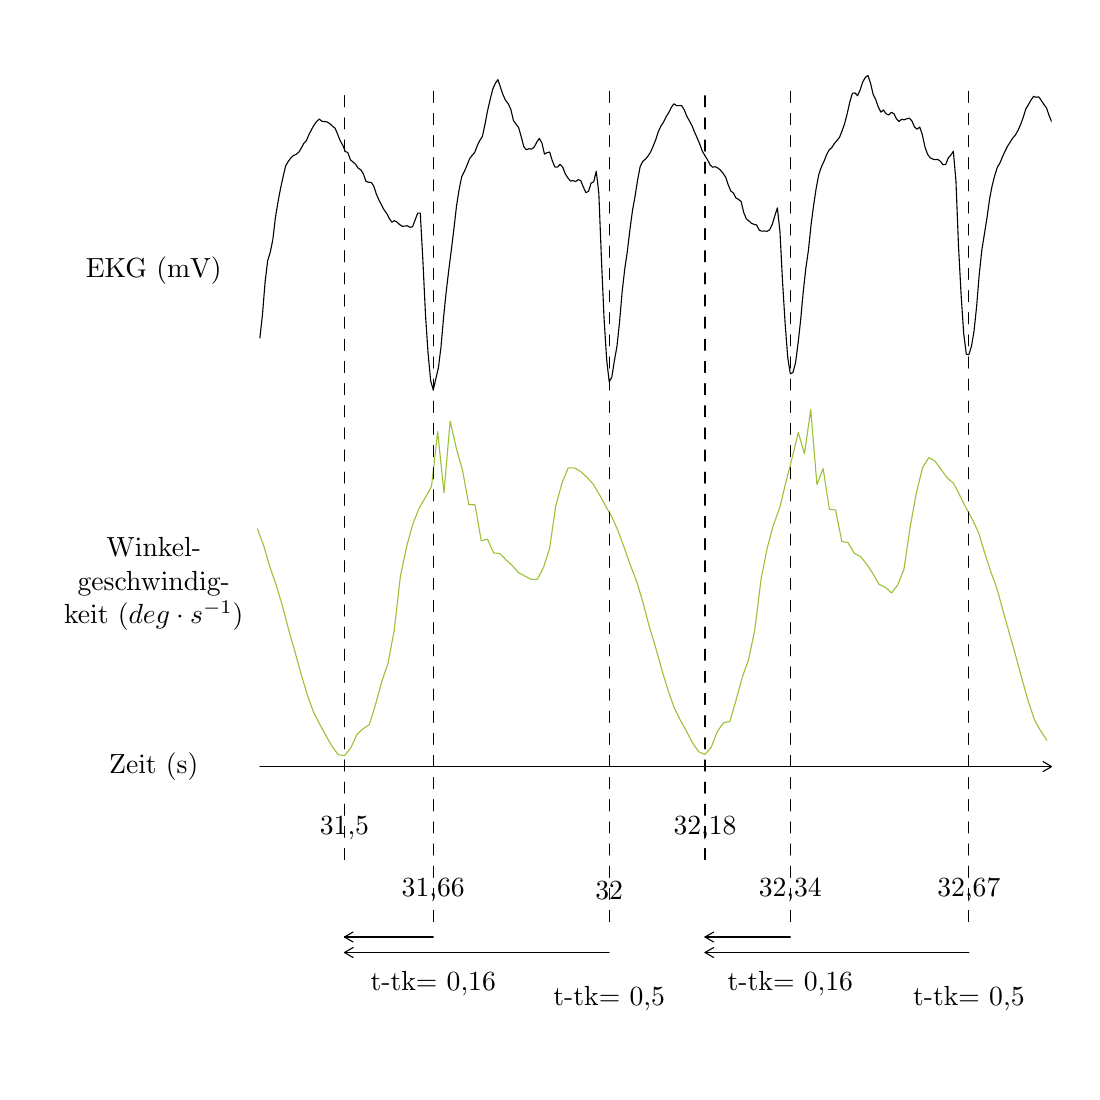
\begin{tikzpicture}[x=1pt,y=1pt]
\definecolor{fillColor}{RGB}{255,255,255}
\path[use as bounding box,fill=fillColor,fill opacity=0.00] (0,0) rectangle (377.25,377.25);
\begin{scope}
\path[clip] (  7.23,  7.23) rectangle (370.02,370.02);
\definecolor{drawColor}{RGB}{0,0,0}

\path[draw=drawColor,line width= 0.4pt,line join=round,line cap=round] ( 83.90,265.09) --
	( 84.84,273.51) --
	( 85.77,285.12) --
	( 86.71,293.00) --
	( 87.64,296.07) --
	( 88.58,300.58) --
	( 89.51,308.54) --
	( 90.45,314.26) --
	( 91.38,319.20) --
	( 92.32,323.51) --
	( 93.25,327.38) --
	( 94.19,328.97) --
	( 95.12,330.21) --
	( 96.06,331.06) --
	( 96.99,331.45) --
	( 97.93,332.22) --
	( 98.86,333.72) --
	( 99.80,335.48) --
	(100.73,336.45) --
	(101.67,338.69) --
	(102.60,340.51) --
	(103.54,342.12) --
	(104.47,343.43) --
	(105.41,344.22) --
	(106.34,343.39) --
	(107.28,343.33) --
	(108.21,343.16) --
	(109.15,342.60) --
	(110.08,341.72) --
	(111.02,341.00) --
	(111.95,338.91) --
	(112.89,336.46) --
	(113.82,334.84) --
	(114.76,332.52) --
	(115.69,332.10) --
	(116.63,329.52) --
	(117.56,328.70) --
	(118.50,327.88) --
	(119.43,326.47) --
	(120.37,325.90) --
	(121.30,324.43) --
	(122.24,321.72) --
	(123.17,321.39) --
	(124.11,321.34) --
	(125.04,320.05) --
	(125.98,317.15) --
	(126.91,315.02) --
	(127.85,313.22) --
	(128.78,311.42) --
	(129.72,310.16) --
	(130.65,308.31) --
	(131.59,306.97) --
	(132.52,307.50) --
	(133.46,306.99) --
	(134.39,306.10) --
	(135.33,305.48) --
	(136.26,305.53) --
	(137.20,305.68) --
	(138.13,305.12) --
	(139.07,305.29) --
	(140.00,307.76) --
	(140.94,310.26) --
	(141.87,310.20) --
	(142.81,293.04) --
	(143.74,273.71) --
	(144.68,259.62) --
	(145.61,249.73) --
	(146.55,246.33) --
	(147.48,250.33) --
	(148.42,254.38) --
	(149.35,261.84) --
	(150.29,272.62) --
	(151.22,281.74) --
	(152.16,289.61) --
	(153.09,296.95) --
	(154.03,304.63) --
	(154.96,312.80) --
	(155.90,318.76) --
	(156.83,323.39) --
	(157.77,325.24) --
	(158.70,327.38) --
	(159.64,329.81) --
	(160.57,331.08) --
	(161.51,332.12) --
	(162.44,334.54) --
	(163.38,336.49) --
	(164.31,337.92) --
	(165.25,342.32) --
	(166.18,347.25) --
	(167.12,351.31) --
	(168.05,355.01) --
	(168.99,357.15) --
	(169.92,358.46) --
	(170.86,355.69) --
	(171.79,352.87) --
	(172.73,350.95) --
	(173.66,349.73) --
	(174.60,347.71) --
	(175.53,343.69) --
	(176.47,342.37) --
	(177.40,341.15) --
	(178.34,337.86) --
	(179.27,334.25) --
	(180.21,333.13) --
	(181.14,333.51) --
	(182.08,333.34) --
	(183.01,334.09) --
	(183.95,335.85) --
	(184.88,337.26) --
	(185.82,335.56) --
	(186.75,331.57) --
	(187.69,332.08) --
	(188.62,332.31) --
	(189.56,329.17) --
	(190.49,326.91) --
	(191.43,326.84) --
	(192.36,327.84) --
	(193.30,326.93) --
	(194.23,324.48) --
	(195.17,323.02) --
	(196.11,321.82) --
	(197.04,321.99) --
	(197.98,321.64) --
	(198.91,322.31) --
	(199.85,322.03) --
	(200.78,319.66) --
	(201.72,317.63) --
	(202.65,318.09) --
	(203.59,321.10) --
	(204.52,321.51) --
	(205.46,325.35) --
	(206.39,317.32) --
	(207.33,293.61) --
	(208.26,272.41) --
	(209.20,257.54) --
	(210.13,249.24) --
	(211.07,250.93) --
	(212.00,256.88) --
	(212.94,262.14) --
	(213.87,270.84) --
	(214.81,281.81) --
	(215.74,289.97) --
	(216.68,296.33) --
	(217.61,304.20) --
	(218.55,311.18) --
	(219.48,316.39) --
	(220.42,322.33) --
	(221.35,327.17) --
	(222.29,329.00) --
	(223.22,329.71) --
	(224.16,330.85) --
	(225.09,332.34) --
	(226.03,334.46) --
	(226.96,336.80) --
	(227.90,339.77) --
	(228.83,341.69) --
	(229.77,343.14) --
	(230.70,345.03) --
	(231.64,346.56) --
	(232.57,348.40) --
	(233.51,349.74) --
	(234.44,349.10) --
	(235.38,349.06) --
	(236.31,349.12) --
	(237.25,347.56) --
	(238.18,345.25) --
	(239.12,343.56) --
	(240.05,341.82) --
	(240.99,339.49) --
	(241.92,337.40) --
	(242.86,335.16) --
	(243.79,332.61) --
	(244.73,331.00) --
	(245.66,329.50) --
	(246.60,327.64) --
	(247.53,326.82) --
	(248.47,327.03) --
	(249.40,326.54) --
	(250.34,325.76) --
	(251.27,324.63) --
	(252.21,323.22) --
	(253.14,320.47) --
	(254.08,318.20) --
	(255.01,317.53) --
	(255.95,315.69) --
	(256.88,315.18) --
	(257.82,314.42) --
	(258.75,310.43) --
	(259.69,308.16) --
	(260.62,307.41) --
	(261.56,306.54) --
	(262.49,306.16) --
	(263.43,305.96) --
	(264.36,304.03) --
	(265.30,303.70) --
	(266.23,303.78) --
	(267.17,303.68) --
	(268.10,304.18) --
	(269.04,306.14) --
	(269.97,309.22) --
	(270.91,312.15) --
	(271.84,303.45) --
	(272.78,285.28) --
	(273.71,270.26) --
	(274.65,258.00) --
	(275.58,252.16) --
	(276.52,252.64) --
	(277.45,256.03) --
	(278.39,263.31) --
	(279.32,271.70) --
	(280.26,281.95) --
	(281.19,290.34) --
	(282.13,296.87) --
	(283.06,305.89) --
	(284.00,313.04) --
	(284.93,319.25) --
	(285.87,324.21) --
	(286.80,326.93) --
	(287.74,328.92) --
	(288.67,331.33) --
	(289.61,333.08) --
	(290.54,333.88) --
	(291.48,335.35) --
	(292.41,336.46) --
	(293.35,337.63) --
	(294.28,339.96) --
	(295.22,342.64) --
	(296.15,346.26) --
	(297.09,350.45) --
	(298.02,353.55) --
	(298.96,353.65) --
	(299.89,352.66) --
	(300.83,354.80) --
	(301.76,357.68) --
	(302.70,359.28) --
	(303.63,359.97) --
	(304.57,357.17) --
	(305.50,353.16) --
	(306.44,351.23) --
	(307.37,348.59) --
	(308.31,346.72) --
	(309.24,347.49) --
	(310.18,346.17) --
	(311.11,345.71) --
	(312.05,346.67) --
	(312.98,346.21) --
	(313.92,344.31) --
	(314.86,343.32) --
	(315.79,344.15) --
	(316.73,343.95) --
	(317.66,344.34) --
	(318.60,344.53) --
	(319.53,343.52) --
	(320.47,341.34) --
	(321.40,340.58) --
	(322.34,341.34) --
	(323.27,338.61) --
	(324.21,334.19) --
	(325.14,331.59) --
	(326.08,330.26) --
	(327.01,329.76) --
	(327.95,329.57) --
	(328.88,329.61) --
	(329.82,328.96) --
	(330.75,327.73) --
	(331.69,327.75) --
	(332.62,330.12) --
	(333.56,331.20) --
	(334.49,332.60) --
	(335.43,321.77) --
	(336.36,298.17) --
	(337.30,280.59) --
	(338.23,266.71) --
	(339.17,259.26) --
	(340.10,259.08) --
	(341.04,262.16) --
	(341.97,267.69) --
	(342.91,276.61) --
	(343.84,288.02) --
	(344.78,296.86) --
	(345.71,302.68) --
	(346.65,308.52) --
	(347.58,315.36) --
	(348.52,320.22) --
	(349.45,323.83) --
	(350.39,326.81) --
	(351.32,328.36) --
	(352.26,330.62) --
	(353.19,332.67) --
	(354.13,334.50) --
	(355.06,335.99) --
	(356.00,337.43) --
	(356.93,338.48) --
	(357.87,340.20) --
	(358.80,342.25) --
	(359.74,344.84) --
	(360.67,347.91) --
	(361.61,349.43) --
	(362.54,351.07) --
	(363.48,352.44) --
	(364.41,352.09) --
	(365.35,352.26) --
	(366.28,350.93) --
	(367.22,349.48) --
	(368.15,348.21) --
	(369.09,345.47) --
	(370.02,343.24);
\end{scope}
\begin{scope}
\path[clip] (  7.23,  7.23) rectangle (370.02,370.02);
\definecolor{drawColor}{RGB}{155,193,54}

\path[draw=drawColor,line width= 0.4pt,line join=round,line cap=round] ( 83.03,196.16) --
	( 85.27,190.13) --
	( 87.52,182.39) --
	( 89.77,175.96) --
	( 92.01,168.47) --
	( 94.26,159.84) --
	( 96.51,151.98) --
	( 98.75,143.84) --
	(101.00,136.30) --
	(103.24,130.07) --
	(105.49,125.59) --
	(107.74,121.48) --
	(109.98,117.57) --
	(112.23,114.52) --
	(114.48,114.23) --
	(116.72,116.92) --
	(118.97,121.89) --
	(121.21,123.88) --
	(123.46,125.43) --
	(125.71,132.72) --
	(127.95,140.94) --
	(130.20,147.54) --
	(132.45,159.51) --
	(134.69,179.10) --
	(136.94,189.76) --
	(139.18,197.91) --
	(141.43,203.57) --
	(143.68,207.44) --
	(145.92,211.47) --
	(148.17,231.26) --
	(150.42,209.19) --
	(152.66,235.08) --
	(154.91,225.19) --
	(157.15,217.21) --
	(159.40,204.91) --
	(161.65,204.83) --
	(163.89,191.84) --
	(166.14,192.41) --
	(168.39,187.44) --
	(170.63,187.24) --
	(172.88,184.92) --
	(175.13,182.84) --
	(177.37,180.32) --
	(179.62,179.14) --
	(181.86,177.92) --
	(184.11,177.83) --
	(186.36,182.11) --
	(188.60,189.15) --
	(190.85,204.59) --
	(193.10,212.77) --
	(195.34,218.19) --
	(197.59,218.15) --
	(199.83,216.84) --
	(202.08,214.77) --
	(204.33,212.32) --
	(206.57,208.58) --
	(208.82,204.46) --
	(211.07,200.47) --
	(213.31,195.47) --
	(215.56,189.36) --
	(217.80,182.96) --
	(220.05,177.18) --
	(222.30,169.69) --
	(224.54,161.14) --
	(226.79,153.73) --
	(229.04,145.59) --
	(231.28,138.18) --
	(233.53,131.70) --
	(235.77,127.14) --
	(238.02,123.07) --
	(240.27,118.79) --
	(242.51,115.58) --
	(244.76,114.64) --
	(247.01,117.29) --
	(249.25,122.99) --
	(251.50,126.08) --
	(253.75,126.57) --
	(255.99,134.35) --
	(258.24,142.61) --
	(260.48,148.88) --
	(262.73,159.55) --
	(264.98,177.83) --
	(267.22,189.19) --
	(269.47,197.54) --
	(271.72,203.65) --
	(273.96,212.93) --
	(276.21,221.73) --
	(278.45,230.93) --
	(280.70,223.28) --
	(282.95,239.28) --
	(285.19,212.16) --
	(287.44,217.90) --
	(289.69,203.20) --
	(291.93,202.96) --
	(294.18,191.60) --
	(296.42,191.19) --
	(298.67,187.32) --
	(300.92,186.18) --
	(303.16,183.37) --
	(305.41,179.99) --
	(307.66,176.08) --
	(309.90,175.02) --
	(312.15,172.99) --
	(314.39,175.84) --
	(316.64,181.54) --
	(318.89,196.89) --
	(321.13,209.19) --
	(323.38,218.31) --
	(325.63,221.89) --
	(327.87,220.59) --
	(330.12,217.49) --
	(332.37,214.48) --
	(334.61,212.57) --
	(336.86,208.13) --
	(339.10,203.69) --
	(341.35,199.62) --
	(343.60,194.77) --
	(345.84,187.36) --
	(348.09,180.52) --
	(350.34,174.25) --
	(352.58,165.99) --
	(354.83,158.05) --
	(357.07,150.11) --
	(359.32,141.76) --
	(361.57,133.78) --
	(363.81,127.18) --
	(366.06,123.07) --
	(368.31,119.73);
\definecolor{drawColor}{RGB}{0,0,0}

\path[draw=drawColor,line width= 0.4pt,dash pattern=on 4pt off 4pt ,line join=round,line cap=round] (114.48, 76.65) -- (114.48,356.59);

\path[draw=drawColor,line width= 0.4pt,dash pattern=on 4pt off 4pt ,line join=round,line cap=round] (244.76, 76.65) -- (244.76,356.59);

\path[draw=drawColor,line width= 0.4pt,dash pattern=on 4pt off 4pt ,line join=round,line cap=round] (146.55, 54.26) -- (146.55,356.59);

\path[draw=drawColor,line width= 0.4pt,dash pattern=on 4pt off 4pt ,line join=round,line cap=round] (210.13, 54.26) -- (210.13,356.59);

\path[draw=drawColor,line width= 0.4pt,dash pattern=on 4pt off 4pt ,line join=round,line cap=round] (275.58, 54.26) -- (275.58,356.59);

\path[draw=drawColor,line width= 0.4pt,dash pattern=on 4pt off 4pt ,line join=round,line cap=round] (340.10, 54.26) -- (340.10,356.59);

\path[draw=drawColor,line width= 0.4pt,line join=round,line cap=round] ( 83.90,110.24) -- (370.02,110.24);

\path[draw=drawColor,line width= 0.4pt,line join=round,line cap=round] (366.89,108.44) --
	(370.02,110.24) --
	(366.89,112.05);

\node[text=drawColor,anchor=base,inner sep=0pt, outer sep=0pt, scale=  1.00] at (114.48, 85.61) {31,5};

\node[text=drawColor,anchor=base,inner sep=0pt, outer sep=0pt, scale=  1.00] at (244.76, 85.61) {32,18};

\node[text=drawColor,anchor=base,inner sep=0pt, outer sep=0pt, scale=  1.00] at (146.55, 63.22) {31,66};

\node[text=drawColor,anchor=base,inner sep=0pt, outer sep=0pt, scale=  1.00] at (210.13, 62.25) {32};

\node[text=drawColor,anchor=base,inner sep=0pt, outer sep=0pt, scale=  1.00] at (275.58, 63.22) {32,34};

\node[text=drawColor,anchor=base,inner sep=0pt, outer sep=0pt, scale=  1.00] at (340.10, 63.22) {32,67};

\node[text=drawColor,anchor=base,inner sep=0pt, outer sep=0pt, scale=  1.00] at ( 45.56,286.90) {EKG (mV)};

\node[text=drawColor,anchor=base,inner sep=0pt, outer sep=0pt, scale=  1.00] at ( 45.56,185.98) {Winkel-};

\node[text=drawColor,anchor=base,inner sep=0pt, outer sep=0pt, scale=  1.00] at ( 45.56,173.98) {geschwindig-};

\node[text=drawColor,anchor=base,inner sep=0pt, outer sep=0pt, scale=  1.00] at ( 45.56,161.98) {keit ($deg \cdot s^{-1}$)};

\node[text=drawColor,anchor=base,inner sep=0pt, outer sep=0pt, scale=  1.00] at ( 45.56,107.74) {Zeit (s)};

\path[draw=drawColor,line width= 0.4pt,line join=round,line cap=round] (146.55, 48.66) -- (114.48, 48.66);

\path[draw=drawColor,line width= 0.4pt,line join=round,line cap=round] (117.60, 50.46) --
	(114.48, 48.66) --
	(117.60, 46.85);

\path[draw=drawColor,line width= 0.4pt,line join=round,line cap=round] (210.13, 43.06) -- (114.48, 43.06);

\path[draw=drawColor,line width= 0.4pt,line join=round,line cap=round] (117.60, 44.87) --
	(114.48, 43.06) --
	(117.60, 41.25);

\path[draw=drawColor,line width= 0.4pt,line join=round,line cap=round] (275.58, 48.66) -- (244.76, 48.66);

\path[draw=drawColor,line width= 0.4pt,line join=round,line cap=round] (247.89, 50.46) --
	(244.76, 48.66) --
	(247.89, 46.85);

\path[draw=drawColor,line width= 0.4pt,line join=round,line cap=round] (340.10, 43.06) -- (244.76, 43.06);

\path[draw=drawColor,line width= 0.4pt,line join=round,line cap=round] (247.89, 44.87) --
	(244.76, 43.06) --
	(247.89, 41.25);

\node[text=drawColor,anchor=base,inner sep=0pt, outer sep=0pt, scale=  1.00] at (146.55, 29.39) {t-tk= 0,16};

\node[text=drawColor,anchor=base,inner sep=0pt, outer sep=0pt, scale=  1.00] at (210.13, 23.79) {t-tk= 0,5};

\node[text=drawColor,anchor=base,inner sep=0pt, outer sep=0pt, scale=  1.00] at (275.58, 29.39) {t-tk= 0,16};

\node[text=drawColor,anchor=base,inner sep=0pt, outer sep=0pt, scale=  1.00] at (340.10, 23.79) {t-tk= 0,5};
\end{scope}
\end{tikzpicture}

	\caption[Grundlage der Berechnung der kardio-lokomotorischen Phasensynchronisation]{Grundlage der Berechnung der kardio-lokomotorischen Phasensynchronisation}
	\label{fig:5_5_grundlage_der_klps}
\end{figure}

Innerhalb eines Zyklus berechnen wir die momentane Phase mit:

\begin{equation}
	\phi(t) = 2 \pi \frac{t-t_{k}}{t_{k+1}-t_{k}} + 2 \pi k,
\end{equation}

wobei $t_{k}$ der Zeit des k-ten Ereignisses entspricht. Die relative Phase für das Auftreten eines Herzschlages bezüglich des Bewegungsablauf berechnen wir demzufolge mit:

\begin{equation}
	\Psi(t_{k}) = 1 \frac{\phi_{L}(t_{k}) \bmod 2 \pi}{2 \pi},
\end{equation}

wobei $t_{k}$ der Zeit des k-ten Auftretens eines Herzschlags und $\phi_{L}$ der momentanen Phase des Bewegungsablaufs entspricht. Stellen wir $\Psi(t_{k})$ über $t_{k}$ dar, erhalten wir das kardio-lokomotorische Synchrogramm. Mit Hilfe des Synchrogramms bin ich in der Lage nachfolgende Aussagen zu treffen:

Sind beiden rhythmischen Oszillatoren unabhängig voneinander, gibt es keine bevorzugte Phase. Die Verteilung von $\Psi(t_{k})$ ist zufällig. Tritt alternativ eine $n:m$ Phasensynchronisation auf, d. h. $\Psi(t_{k})$ tritt genau zu den gleichen $n$ Werten innerhalb der $m$ Bewegungsablauf auf, beobachten wir $n$ parallele horizontale Linien.

Die visuelle Bestimmung der Synchronität erfolgt über ein R-Programm. Das Programm berechnet zusätzlich den Phasenkohärenz Index \citep{Rosenblum2003} und den normalisierten Shannon Entropie Index \citep{Tass1998, Niizeki2005} zur Quantifizierung der kardio-lokomotorischen Phasensynchronisation und stellt sie dar. Indizes und Phasen sichert das Programm in einer Textdatei im \acs{csv}-Format.

% paragraph r_programme_zur_erkennung (end)

% subsubsection psychophysiopipeline (end)

% subsection apparat (end)

\subsection{Operationalisierung und gewonnene Daten} % (fold)
\label{sub:operationalisierung_und_gewonnene_daten}

\subsubsection{Selbstauskünfte} % (fold)
\label{ssub:selbstauskunfte}

Auf der Grundlage der sechs Sitzungen erhielt ich 24 Selbstauskünfte durch die Befragung mit der \ac{FKS}. Die \ac{FKS} besitzt nach \citet{Rheinberg2003} eine hohe Güte. Nichtsdestotrotz überprüfte ich die gewonnenen Daten nochmals auf ihre Eignung. Ich garantiere damit, dass die aus der Skala ermittelten Messwerte, die zu beschreibenden Faktoren mit hoher Reliabilität wiedergeben. Gleichzeitig prüfe ich, ob ich die \ac{FKS} im vorliegenden Einzelfall einer laufenden Person erfolgreich eingesetzt habe.

Zur Verifizierung betrachtete ich die 24 Selbstauskünfte und bestimmte den Mittelwert und die Standardabweichung jedes Items des Generalfaktors und der beiden Faktoren der \ac{FKS}. Ebenso berechnete ich für jeden Faktor und dessen Items die Item-Faktor-Korrelation. Die Item-Faktor-Korrelation dient häufig als Testgröße der Trennschärfe. Je höher und gleichmäßiger die Trennschärfe ist, desto höher ist die Konsistenz zwischen den Items und desto besser die verwendete Skala. Als Daumenregel gilt, eine Trennschärfe von größer als 0,5 ist passend. Solange die Items nur geringfügig unter 0,5 liegen, sieht man sie als vertretbar an. Wichtig ist in jedem Fall, dass keine der Trennschärfen signifikant von allen übrigen abweicht und dass die Trennschärfen niemals negativ sind \citep[][S.~219f.]{Bortz2006}.

Neben der Trennschärfe der einzelnen Items bestimmte ich für die Faktoren der \ac{FKS} die Maßzahl Cronbachs~$\alpha$, um festzustellen, inwieweit ich die Faktoren zur Messung der einzelnen latenten Wirkungsdimensionen heranziehen kann. Das Cronbachs~$\alpha$ ist eine in den Wirtschafts- und Sozialwissenschaften häufig verwendetes Reliabilitätskriterium in der Testkonstruktion und -evaluation. Vernünftige Werte für das Cronbachs~$\alpha$ sind größer 0,7 \citep[][S.~189f.]{Bortz2006}.

Die Reliabilität des Generalfaktors und der Absorbiertheit weisen mit 0,81 und 0,77 auf eine gute Eignung hin. Die Reliabilität des glatten Verlaufs ist mit 0,68 akzeptabel. Die Trennschärfen sind bis auf die Items „Mein Kopf ist völlig klar.“ und „Ich weiß bei jedem Schritt, was ich zu tun habe.“ für den Generalfaktor, bei denen die Trennschärfe unter 0,4 liegt, akzeptabel (Tabellen~\ref{tab:generalfaktor_erste_studie_laufen}, \ref{tab:glatter_verlauf_erste_studie_laufen} und \ref{tab:absorbiertheit_erste_studie_laufen}). In der Untersuchung hatte das Ergebnis für die Items keine Konsequenzen, da es sich bei \ac{FKS} um eine wissenschaftlich eingehend untersuchte Skala handelt und da ich mögliche inhaltliche Verfälschungen durch weglassen von Items vermeiden wollte.

% subsubsection selbstauskunfte (end)

% subsection operationalisierung_und_gewonnene_daten (end)

% section methode (end)

% section flow_und_laufen_intraindividuell (end)